% !TeX program = lualatex
% SPDX-License-Identifier: GPL-3.0-or-later
% SPDX-FileCopyrightText: 2026 William W. Wallace <wwallace@nrao.edu>
% SPDX-FileCopyrightText: 2026 William W. Wallace, Adaptive Electrodynamics LLC dba AdaptEd
% =============================================================================
%    FILE HEADER
% =============================================================================
%  Title          : EMF Envelope FFT Analyzer - User Manual
%  Filename       : EMF_Envelope_FFT_Manual_v0.0.2.tex
%  Version        : 0.0.2 (Semantic Versioning 2.0.0; follows the program)
%  Author         : William W. Wallace
%  Company        : NRAO/GBO
%  Email          : wwallace@nrao.edu
%  Created        : 2026-10-15
%  Modified       : 2026-10-15
%  Language       : LaTeX for LuaLaTeX (LuaHBTeX), TeX Live 2023+ or MiKTeX
%  Requires       : fontspec, unicode-math, amsmath, hyperref, bookmark,
%                   booktabs, longtable, array, fvextra, fancyhdr, graphicx,
%                   caption, float, enumitem, xcolor, url, tocloft; DejaVu fonts
%                   (Latin Modern is used when DejaVu is not installed)
%  Licence        : GPL-3.0-or-later (GNU General Public License v3.0 or later)
%  Copyright      : Copyright (C) 2026 William W. Wallace
%  Generated by   : tools/build_manual_pdf.py 0.0.2. Edit that script, not
%                   this file: the next build overwrites this file.
%  Build          : lualatex EMF_Envelope_FFT_Manual_v0.0.2.tex   (three runs: contents,
%                   longtable widths, bookmarks), or run the build tool.
%  Bookmarks      : every \section and \subsection (appendices and references
%                   included) becomes a numbered PDF bookmark (hyperref +
%                   bookmark); the bookmark pane opens with the PDF.
% =============================================================================

% =============================================================================
%    PREAMBLE
% =============================================================================
\documentclass[10pt,letterpaper]{article}
\usepackage[margin=2.0cm,headheight=14pt]{geometry}

% ---- fonts: DejaVu when installed (TeX Live ships it), else Latin Modern ----
\usepackage{amsmath}
\usepackage{unicode-math}
\IfFontExistsTF{DejaVu Serif}{%
  \setmainfont{DejaVu Serif}%
  \setsansfont{DejaVu Sans}%
  \setmonofont[Scale=0.85]{DejaVu Sans Mono}}{}
\IfFontExistsTF{DejaVu Math TeX Gyre}{\setmathfont{DejaVu Math TeX Gyre}}{\setmathfont{Latin Modern Math}}

% ---- layout, tables, figures, code ------------------------------------------
\usepackage{xcolor}
\usepackage{graphicx}
\usepackage{array,booktabs,longtable}
\usepackage[font=small,labelfont=bf]{caption}
\usepackage{float}
\usepackage{enumitem}
\usepackage{fvextra}
\usepackage{fancyhdr}
\usepackage{url}
\def\UrlBreaks{\do\/\do\_\do\-\do\.\do\=\do\&}
\newcolumntype{L}[1]{>{\raggedright\arraybackslash}p{#1}}
\fvset{breaklines,breakanywhere,fontsize=\small,frame=leftline,framerule=0.6pt,rulecolor=\color{gray}}
\setlist{itemsep=1pt,topsep=3pt}
\setlength{\parskip}{3pt}
\setlength{\parindent}{0pt}
\sloppy
\renewcommand{\arraystretch}{1.12}
\usepackage[titles]{tocloft}            % wider number boxes: "10" and "5.10" fit
\setlength{\cftsecnumwidth}{2.0em}
\setlength{\cftsubsecnumwidth}{2.9em}
\setlength{\cfttabnumwidth}{2.3em}
\setlength{\cftfignumwidth}{2.3em}
\numberwithin{equation}{section}
\DeclareMathOperator{\sinc}{sinc}

% ---- header and footer -----------------------------------------------------------
\pagestyle{fancy}
\fancyhf{}
\lhead{\small EMF Envelope FFT Analyzer --- User Manual}
\rhead{\small\thepage}
\lfoot{\scriptsize Version 0.0.2 (2026-10-15), GPL-3.0-or-later}
\rfoot{\scriptsize W.\,W.\ Wallace, NRAO/GBO}

% ---- hyperlinks and heading-based PDF bookmarks (load last) --------------------
\usepackage[bookmarks=true,bookmarksnumbered=true,bookmarksopen=true,
            bookmarksopenlevel=1,pdfpagemode=UseOutlines,colorlinks=true,
            linkcolor=blue!50!black,citecolor=green!40!black,
            urlcolor=blue!60!black]{hyperref}
\usepackage{bookmark}
\bookmarksetup{numbered,open,openlevel=1}
\hypersetup{
  pdftitle={EMF Envelope FFT Analyzer - User Manual, version 0.0.2},
  pdfauthor={William W. Wallace, NRAO/GBO},
  pdfsubject={Envelope (modulation) spectra of Narda broadband probe and SignalShark logs},
  pdfkeywords={EMF, envelope FFT, Welch, chirp-Z, Lomb-Scargle, Narda, FieldMan, SignalShark, Veusz},
  pdfcreator={tools/build_manual_pdf.py 0.0.2 with LuaLaTeX}}

% =============================================================================
%    FRONT MATTER
% =============================================================================
\begin{document}
\begin{titlepage}
\pdfbookmark[section]{Title page}{titlepage}
\centering
\vspace*{3cm}
{\Huge\bfseries EMF Envelope FFT Analyzer\par}
\vspace{0.6cm}
{\Large User Manual\par}
\vspace{1.2cm}
{\large Envelope (modulation) spectra of broadband EMF probe logs\\
(FieldMan / Narda-TSX, NBM-550, EHP-50 TS) and SignalShark spectrograms\par}
\vspace{1.5cm}
{\large Program version 0.0.2 \quad$\cdot$\quad vszh5\_writer 0.0.11 \quad$\cdot$\quad 2026-10-15\par}
\vspace{2cm}
{\large William W. Wallace\par}
NRAO/GBO\\
\href{mailto:wwallace@nrao.edu}{wwallace@nrao.edu}\par
\vfill
{\small Copyright \copyright{} 2026 William W. Wallace (Adaptive Electrodynamics LLC dba AdaptEd).\\
This manual and the programs it describes are free software under the\\
GNU General Public License v3.0 or later (GPL-3.0-or-later).\par}
\vspace{0.5cm}
{\small\itshape Internal draft: tested on synthetic files only (Section~\ref{sec:verification}).\par}
\end{titlepage}

\pdfbookmark[section]{Contents}{contents}
\tableofcontents
\clearpage
\pdfbookmark[section]{List of tables}{lot}
\listoftables
\pdfbookmark[section]{List of figures}{lof}
\listoffigures
\clearpage

% =============================================================================
%    1  INTRODUCTION
% =============================================================================
\section{Introduction}\label{sec:intro}

A broadband diode probe such as the Narda EFD-4091, EFD-0691, EF\,0691 or
EFD-9091 adds the power of every source in its frequency range and reports one
number per sample \cite{R1,R2,R3}. Its log therefore holds no information about
the radio frequency of a source. It does hold how the total field changes in
time: a radar antenna rotating, a beam being scanned, a transmitter keyed on and
off, a duty cycle. The \emph{EMF Envelope FFT Analyzer} takes the Fourier
transform of that envelope, the \emph{modulation spectrum}, so that sources which
share an RF band but change at different rates can be told apart and their rates
measured (a rotating antenna appears as a line at its rotation frequency, with
harmonics from the beam shape).

The program reads the files written by the software of the instruments in use:
FieldMan and Narda-TSX exports for the EFD probes \cite{R5,R9}, NBM-550 or
NBM-TS logs for the EF\,0691 probe \cite{R6}, EHP-50 TS spectra of the EHP-50F
low-frequency analyzer \cite{R7}, and SignalShark spectrum or spectrogram files
\cite{R8}. A SignalShark spectrogram, unlike a probe log, does resolve RF
frequency; for it the envelope transform is taken for every frequency bin.

\subsection{What the analysis can and cannot tell you}
\begin{itemize}
\item \textbf{Can}: the rates at which the total field changes (rotation in rpm,
scan or keying periods), the relative strength of each modulation, and which
modulations come from the same source (harmonic families).
\item \textbf{Cannot}: the RF frequency of a source measured with a diode probe;
content faster than half the probe's sample rate (it folds back, Section~\ref{sec:sinc});
an exposure assessment, for which IEC~62232 \cite{R18} and calibrated probes
(IEEE~1309 \cite{R17}) remain the reference.
\item \textbf{Only partly}: content near the Nyquist frequency is attenuated by
the probe's own averaging; the program models and can partly undo that
(Section~\ref{sec:correction}).
\end{itemize}

\subsection{Status of this version}
Version 0.0.2 is an internal draft. No real export of FieldMan,
Narda-TSX, NBM-TS, EHP-50 TS or SignalShark has been available yet, so the
readers recognise file layouts by heuristics (Section~\ref{sec:inputs}) and
were tested on synthetic files written in the expected styles. Use
\texttt{--inspect} on every new kind of file before trusting an analysis, and
see Section~\ref{sec:limits} for the known limitations.

\subsection{Conventions}
\begin{itemize}
\item $f$ is an RF (or spectrum) frequency, $\nu$ an envelope (modulation)
frequency; $f_s$ is the sample rate of the log, $N$ the number of samples, and
$T$ the probe's integration time.
\item $\sinc x = \sin(\pi x)/(\pi x)$, the normalised form used by NumPy.
\item Versions follow Semantic Versioning (\texttt{X.Y.Z}); the manual carries
the version of the program it documents.
\item Commands are shown for a Windows or Linux shell inside the mamba
environment; \texttt{python} is the environment's interpreter.
\end{itemize}

% =============================================================================
%    2  INSTALLATION
% =============================================================================
\section{Installation}\label{sec:install}

\subsection{Mamba environment}
The environment file creates an environment named \texttt{emf-fft} from
conda-forge with Python~3.12 and every dependency \cite{B36}:
\begin{Verbatim}
mamba env create -f emf_envelope_fft.yml
mamba activate emf-fft
python emf_envelope_fft_v0_0_2.py --selftest
\end{Verbatim}
The self-test (Section~\ref{sec:verification}) must end with
\texttt{SELF-TEST PASSED}. For a GPU (NVIDIA CUDA only), also install CuPy
(\texttt{mamba install -c conda-forge cupy}) and add \texttt{--gpu}.

\subsection{Package files}
Keep the files together as delivered; \path{vszh5_writer.py} must sit in the
same folder as the script, which puts its own folder first on the module search
path so that this copy is used rather than an older one (e.g.\ from the
QuickSyn package). Table~\ref{tab:files} lists the package.

\begingroup\small
\begin{longtable}{@{}L{\dimexpr 0.3\linewidth-2\tabcolsep\relax}L{\dimexpr 0.16\linewidth-2\tabcolsep\relax}L{\dimexpr 0.1\linewidth-2\tabcolsep\relax}L{\dimexpr 0.4\linewidth-2\tabcolsep\relax}@{}}
\caption{Files of the package.}\label{tab:files}\\
\toprule
\textbf{File} & \textbf{Type} & \textbf{Size} & \textbf{Description} \\
\midrule
\endfirsthead
\multicolumn{4}{@{}l}{\itshape\footnotesize Table \thetable{} (continued)}\\
\toprule
\textbf{File} & \textbf{Type} & \textbf{Size} & \textbf{Description} \\
\midrule
\endhead
\bottomrule
\endlastfoot
\path{emf_envelope_fft_v0_0_2.py} & Python 3.12 script & 3031 lines & The analyzer: readers, estimators, Veusz/CSV/JSON output, batch, live mode, self-test. Spyder cells (Table \ref{tab:cells}). \\
\path{vszh5_writer.py} & Python module & 1209 lines & The author's Veusz HDF5 writer, 0.0.11: typed datasets, 2-D images, plot-page helpers, rendering to PDF (with bookmarks) and PNG. Must stay next to the script. \\
\path{emf_envelope_fft.yml} & mamba environment & -- & Creates the environment emf-fft from conda-forge (Python 3.12 and every dependency; CuPy commented out). \\
\path{LICENSE} & text & -- & GNU General Public License v3.0. \\
\path{docs/EMF_Envelope_FFT_Manual_v0.0.2.pdf} & PDF & -- & This manual, with heading-based bookmarks. \\
\path{docs/EMF_Envelope_FFT_Manual_v0.0.2.tex} & LuaLaTeX source & -- & Source of this manual; written by the build tool, compiles on its own with lualatex. \\
\path{docs/figures/*.png} & PNG & -- & Figures of this manual: Veusz pages rendered from the self-test's synthetic files, and screenshots of the live window. \\
\path{tools/build_manual_pdf.py} & Python 3.12 script & 1948 lines & Builds this manual (generated tables, self-test run, LuaLaTeX, bookmark check). \\
\end{longtable}
\endgroup


\subsection{Veusz and LuaLaTeX (optional)}
The \texttt{.vszh5} documents are written without Veusz; Veusz is needed only
to open them or to render them with \texttt{--render} \cite{B23}. The renderer
finds Veusz on the PATH, in the usual install folders, or through the
environment variable \texttt{VEUSZ\_EXE} (or \texttt{QUICKSYN\_VEUSZ}), e.g.\
\verb|set VEUSZ_EXE=C:\Program Files\Veusz\veusz.exe|. Rebuilding this manual
needs \texttt{lualatex} from TeX~Live or MiKTeX (or \texttt{EMF\_FFT\_LUALATEX}
pointing to it); its headings become the PDF bookmarks through hyperref and bookmark \cite{B37}.

\subsection{Spyder}
Select the interpreter of the \texttt{emf-fft} environment in Spyder
(\emph{Tools $\rightarrow$ Preferences $\rightarrow$ Python interpreter}; the
environment includes \texttt{spyder-kernels}) \cite{B35}. The script is
divided into \verb|# %%| cells (Section~\ref{sec:spyder}); run them in order
with \emph{Run cell}, then use the scratch cell at the end.

% =============================================================================
%    3  QUICK START
% =============================================================================
\section{Quick start}\label{sec:quickstart}

\begin{Verbatim}
:: 1  check the installation
python emf_envelope_fft_v0_0_2.py --selftest

:: 2  see how a file will be read (columns, units, time base)
python emf_envelope_fft_v0_0_2.py --inspect export.csv

:: 3  analyse one probe log; also render PDF and PNG with Veusz
python emf_envelope_fft_v0_0_2.py export.csv --probe EFD-4091 --render

:: 4  undo the probe's averaging and force Lomb-Scargle
python emf_envelope_fft_v0_0_2.py export.csv --probe EFD-4091 --correct-probe --lomb on

:: 5  several files in parallel, on the GPU if one is available
python emf_envelope_fft_v0_0_2.py a.csv b.csv c.csv --jobs 3 --gpu

:: 6  SignalShark spectrogram, the five strongest carriers as channels
python emf_envelope_fft_v0_0_2.py rec.h5 --source signalshark --rf-channels auto:5

:: 7  EHP-50 TS: the whole folder of auto-saved spectra
python emf_envelope_fft_v0_0_2.py D:\EHP50\2026 --source ehp

:: 8  follow a file that another program is writing (live window)
python emf_envelope_fft_v0_0_2.py --live growing.csv --probe EF0691 --window-s 120
\end{Verbatim}

\subsection{Typical workflow}
\begin{enumerate}
\item Export the measurement from the instrument software as text (CSV/TXT) or
Excel, or copy the SignalShark \texttt{.h5} file.
\item Run \texttt{--inspect} and check the detected delimiter, decimal mark,
columns, unit and sample interval. Correct anything wrong with the override
options (Section~\ref{sec:overrides}).
\item Run the analysis with \texttt{--probe} set, so that the sample rate,
integration time and range limits of the probe are known.
\item Open \path{<stem>_envelope_fft.vszh5} in Veusz, or use the rendered PDF,
whose bookmarks list every page (Section~\ref{sec:outputs}).
\item Read \path{<stem>_summary.json}: peaks, harmonic families with their rpm,
and warnings about timing, gaps, aliasing and range.
\end{enumerate}

% =============================================================================
%    4  INSTRUMENTS AND INPUT FILES
% =============================================================================
\section{Instruments and input files}\label{sec:inputs}

\subsection{Probe catalogue}
Table~\ref{tab:probes} lists the probes the program knows, from the
datasheets. \texttt{--probe} accepts the names in the first column (case and
spaces ignored) and the aliases \texttt{EFD-4091E} (treated as the EFD-4091;
no separate datasheet for an ``E'' variant was found), \texttt{EF-0691},
\texttt{EFD-1891FAST} and the forms without hyphens. The last four columns are
derived: the Nyquist frequency $f_s/2$, the response of the probe's averaging at
that frequency, and the first null $1/T$ of that response
(Section~\ref{sec:sinc}).

\begingroup\footnotesize
\begin{longtable}{@{}L{\dimexpr 0.14\linewidth-2\tabcolsep\relax}L{\dimexpr 0.13\linewidth-2\tabcolsep\relax}L{\dimexpr 0.07\linewidth-2\tabcolsep\relax}L{\dimexpr 0.1\linewidth-2\tabcolsep\relax}L{\dimexpr 0.08\linewidth-2\tabcolsep\relax}L{\dimexpr 0.1\linewidth-2\tabcolsep\relax}L{\dimexpr 0.08\linewidth-2\tabcolsep\relax}L{\dimexpr 0.1\linewidth-2\tabcolsep\relax}L{\dimexpr 0.08\linewidth-2\tabcolsep\relax}L{\dimexpr 0.08\linewidth-2\tabcolsep\relax}@{}}
\caption{Probe catalogue (datasheet values) and the derived envelope limits.}\label{tab:probes}\\
\toprule
\textbf{Probe} & \textbf{RF range} & \textbf{$f_s$ (Hz)} & \textbf{$T$ (ms)} & \textbf{$\nu_N$ (Hz)} & \textbf{$|H(\nu_N)|$ (dB)} & \textbf{$1/T$ (Hz)} & \textbf{True RMS to (V/m)} & \textbf{Axes} & \textbf{Ref.} \\
\midrule
\endfirsthead
\multicolumn{10}{@{}l}{\itshape\footnotesize Table \thetable{} (continued)}\\
\toprule
\textbf{Probe} & \textbf{RF range} & \textbf{$f_s$ (Hz)} & \textbf{$T$ (ms)} & \textbf{$\nu_N$ (Hz)} & \textbf{$|H(\nu_N)|$ (dB)} & \textbf{$1/T$ (Hz)} & \textbf{True RMS to (V/m)} & \textbf{Axes} & \textbf{Ref.} \\
\midrule
\endhead
\bottomrule
\endlastfoot
EFD-4091\newline\footnotesize 2462/19 & 2 MHz -\kern0pt- 40 GHz & 5 & 265 & 2.5 & -7.6 & 3.774 & 65 & rss & \cite{R1} \\
EFD-0691\newline\footnotesize 2462/14B & 100 kHz -\kern0pt- 6 GHz & 5 & 265 & 2.5 & -7.6 & 3.774 & 17 & xyz & \cite{R2} \\
EF 0691 (NBM)\newline\footnotesize NBM probe & 100 kHz -\kern0pt- 6 GHz & 5 & n/p\newline\footnotesize(1/fs used) & 2.5 & -3.9 & 5 & 22 & rss & \cite{R6} \\
EFD-9091\newline\footnotesize 2462/18 & 100 MHz -\kern0pt- 90 GHz & 5 & 275 & 2.5 & -8.3 & 3.636 & 61.4 & rss & \cite{R3} \\
EFD-1891 Fast\newline\footnotesize 2462/23 & 2 MHz -\kern0pt- 18 GHz & 900 & 2.3 & 450 & -29.4 & 434.8 & -- & rss & \cite{R4} \\
\end{longtable}
\endgroup


\subsection{Readers}
The reader is chosen from the file (Table~\ref{tab:readers}); \texttt{--source}
forces one.

\begingroup\small
\begin{longtable}{@{}L{\dimexpr 0.14\linewidth-2\tabcolsep\relax}L{\dimexpr 0.22\linewidth-2\tabcolsep\relax}L{\dimexpr 0.16\linewidth-2\tabcolsep\relax}L{\dimexpr 0.24\linewidth-2\tabcolsep\relax}L{\dimexpr 0.2\linewidth-2\tabcolsep\relax}@{}}
\caption{Readers and how the input is recognised.}\label{tab:readers}\\
\toprule
\textbf{\texttt{--source}} & \textbf{Instrument / software} & \textbf{Files} & \textbf{Auto-detected when} & \textbf{Result} \\
\midrule
\endfirsthead
\multicolumn{5}{@{}l}{\itshape\footnotesize Table \thetable{} (continued)}\\
\toprule
\textbf{\texttt{--source}} & \textbf{Instrument / software} & \textbf{Files} & \textbf{Auto-detected when} & \textbf{Result} \\
\midrule
\endhead
\bottomrule
\endlastfoot
\texttt{fieldman, tsx} & FieldMan or Narda-TSX with EFD-4091, -0691, -9091, -1891 & .csv .txt & default for text files & time series (+ X/Y/Z) \\
\texttt{nbm} & NBM-550 / NBM-TS with EF 0691 & .csv .txt & a column named 'Result ...' & time series \\
\texttt{xlsx} & any of the above saved as Excel & .xlsx .xls & by extension & time series \\
\texttt{ehp} & EHP-50 TS with EHP-50F (1 Hz - 400 kHz) & folder, \path{hh_mm_ss_cc.TXT} & a folder, or the EHP file name & spectrogram (folder), spectrum, or time series (logger file) \\
\texttt{signalshark} & SignalShark & .h5 .hdf5; converter .csv & .h5 extension; 8+ numeric column names or a frequency column & spectrogram (or level time series) \\
\end{longtable}
\endgroup


\subsection{How text exports are read}\label{sec:textreading}
Narda's software is German-made, so semicolon-separated files with a decimal
comma are expected as often as comma-separated files with a decimal point.
\begin{enumerate}
\item \textbf{Encoding}: UTF-8 (with or without byte-order mark), then
Windows-1252, then Latin-1.
\item \textbf{Delimiter}: the first of tab, \texttt{;}, \texttt{,}, \texttt{|}
that occurs the same number of times on the last 50 non-blank lines;
whitespace otherwise. Semicolon is tried before comma because a decimal comma
puts a comma inside every number.
\item \textbf{Decimal mark}: comma when numbers such as \texttt{1,23} appear
and the delimiter is not a comma.
\item \textbf{Header row}: the first row with the same number of fields as the
row below it and more text fields than that row, whose fields are mostly
numbers or date/times. Lines above it are kept as metadata and searched for a
unit.
\item \textbf{Columns}: chosen with the keyword lists of Table~\ref{tab:keywords};
the unit comes from \texttt{--unit}, the value column's header or the
metadata, in that order.
\item \textbf{Time}: numbers are seconds (milliseconds when the header says
\texttt{ms}); anything else is parsed as date/time, day first when dates look
like \texttt{dd.mm.yyyy}. A date column and a clock column are joined. The
first value is the origin of every chunk of a large file, so the time axis is
continuous.
\item \textbf{Size}: the file is read in chunks of 500\,000 rows; columns longer
than 20\,000\,000 samples move to a temporary file on disk (Section~\ref{sec:memory}).
\end{enumerate}

\begingroup\footnotesize
\begin{longtable}{@{}L{\dimexpr 0.2\linewidth-2\tabcolsep\relax}L{\dimexpr 0.46\linewidth-2\tabcolsep\relax}L{\dimexpr 0.3\linewidth-2\tabcolsep\relax}@{}}
\caption{Keywords that select columns (case ignored).}\label{tab:keywords}\\
\toprule
\textbf{Use} & \textbf{Keywords} & \textbf{Note} \\
\midrule
\endfirsthead
\multicolumn{3}{@{}l}{\itshape\footnotesize Table \thetable{} (continued)}\\
\toprule
\textbf{Use} & \textbf{Keywords} & \textbf{Note} \\
\midrule
\endhead
\bottomrule
\endlastfoot
time column & \texttt{time}, \texttt{zeit}, \texttt{uhrzeit}, \texttt{timestamp}, \texttt{date}, \texttt{datum}, \texttt{elapsed}, \texttt{t [s]}, \texttt{t(s)}, \texttt{t/s}, \texttt{sec}, \texttt{hh:mm} & a date column and a clock column are joined; otherwise the first match \\
value column, preferred (+5) & \texttt{actual}, \texttt{act}, \texttt{rss}, \texttt{total}, \texttt{result 1}, \texttt{isotrop}, \texttt{value}, \texttt{wert}, \texttt{e-field}, \texttt{e field}, \texttt{field}, \texttt{level} & +3 more if the header names a unit; leftmost column wins ties \\
value column, avoided (-6) & \texttt{max}, \texttt{min}, \texttt{avg}, \texttt{mean}, \texttt{average}, \texttt{batt}, \texttt{temp}, \texttt{humid}, \texttt{press}, \texttt{lat}, \texttt{lon}, \texttt{alt}, \texttt{gps}, \texttt{index}, \texttt{no.}, \texttt{nr}, \texttt{flag}, \texttt{dist}, \texttt{comment} & statistics and house-keeping columns \\
axis columns & \texttt{X, Y, Z, E\_x, H y, field\_z, ...} & used for per-axis spectra; their RSS is the value when no value column exists \\
\end{longtable}
\endgroup


\subsection{EHP-50 TS spectra}
EHP-50 TS saves one spectrum per file as \path{YYYY/MM/DD/hh_mm_ss_cc.TXT}
($cc$ = hundredths of a second) \cite{R7}. Given a folder, the program reads
every \texttt{.txt}/\texttt{.csv} below it, takes the time of each spectrum from
its path (the file date when the name does not match), sorts them, and puts
every spectrum on the frequency axis of the first one (linear interpolation
when they differ). The total or RSS column is preferred over X, Y, Z. The result
is analysed as a spectrogram (Section~\ref{sec:spectrogram}). Note that EHP-50 TS
records only the EHP-50F (1\,Hz to 400\,kHz); it cannot record the RF probes.

\subsection{SignalShark files}
The layout of SignalShark's \texttt{.h5} files is not published. The reader
takes the largest two-dimensional numeric dataset as levels (time $\times$
frequency, transposed if the axes say so), a one-dimensional dataset of matching
length whose name or values look like frequencies as the frequency axis, and one
that increases as the time axis; otherwise start/stop/centre/span and
time-resolution attributes. \texttt{--h5-level}, \texttt{--h5-freq} and
\texttt{--h5-time} name the datasets explicitly; \texttt{--inspect} prints the
whole HDF5 tree. CSV files made with Narda's NSL \emph{Converter} script
\cite{R8} are read in wide format (one row per spectrum, the header holding the
frequencies), long format (time, frequency, level columns) or transposed wide
format (one row per frequency). Levels in dBm or dB\textmu V are converted to
field strength only when an antenna factor is given (\texttt{--antenna-factor-db}).

\subsection{Overriding the detection}\label{sec:overrides}
\texttt{--source}, \texttt{--time-col} (\texttt{"Date+Time"} joins two columns),
\texttt{--value-col}, \texttt{--unit}, \texttt{--sep}, \texttt{--decimal},
\texttt{--dayfirst} and \texttt{--fs} (for files without a time column) override
the corresponding guess. Column names or zero-based indices are accepted.

% =============================================================================
%    5  THEORY AND METHODS
% =============================================================================
\section{Theory and methods}\label{sec:theory}

\subsection{Square-law detection adds powers}\label{sec:powersum}
A diode detector operated in its square-law region delivers a voltage
proportional to the square of the RF voltage. Let the field at the probe be the
sum of $M$ sources,
\begin{equation}
E(t) = \sum_{i=1}^{M} E_i \cos(2\pi f_i t + \varphi_i).
\end{equation}
The detector output, averaged by a video filter that is much slower than any
difference frequency $|f_i - f_j|$, is
\begin{align}
\overline{E^2} &= \sum_{i}\sum_{j} E_i E_j\,\overline{\cos(2\pi f_i t+\varphi_i)\cos(2\pi f_j t+\varphi_j)} \nonumber\\
&= \sum_{i}\sum_{j} \frac{E_i E_j}{2}\Big[\overline{\cos\big(2\pi(f_i-f_j)t+\varphi_i-\varphi_j\big)}
 + \overline{\cos\big(2\pi(f_i+f_j)t+\varphi_i+\varphi_j\big)}\Big] \nonumber\\
&= \sum_{i} \frac{E_i^2}{2} = \sum_i E_{i,\mathrm{rms}}^2,
\label{eq:powersum}
\end{align}
because every term with $i\neq j$ and every sum-frequency term averages to
zero. Three orthogonal sensors add in the same way,
$E^2 = E_x^2 + E_y^2 + E_z^2$ (the isotropic RSS value). With the probe's
frequency response $r(f)$ and the plane-wave power density
$S = E_\mathrm{rms}^2 / Z_0$, the displayed value is
\begin{equation}
S_\mathrm{disp}(t) = \sum_i r(f_i)\, S_i(t),\qquad
E_\mathrm{disp}(t) = \sqrt{Z_0\, S_\mathrm{disp}(t)}.
\label{eq:sdisp}
\end{equation}
Equation~\eqref{eq:powersum} holds only while every diode stays in its
square-law region, which for the EFD probes is the True-RMS range of
Table~\ref{tab:probes}; above it the program warns.

\subsection{Why the transform is taken of power}\label{sec:whypower}
The Fourier transform is linear, so applying it to \eqref{eq:sdisp} gives
\begin{equation}
\mathcal{F}\{S_\mathrm{disp}\}(\nu) = \sum_i r(f_i)\,\mathcal{F}\{S_i\}(\nu):
\label{eq:linear}
\end{equation}
the envelope spectrum of the log is the weighted sum of the envelope spectra of
the sources, and each source's modulation lines appear unchanged. The field
$E_\mathrm{disp} = \sqrt{Z_0 S_\mathrm{disp}}$ does not have this property. Take
two sources $S_1 = a + b\cos 2\pi\nu_1 t$ and $S_2 = c + d\cos 2\pi\nu_2 t$ with
$A = a+c$ and $x(t) = b\cos 2\pi\nu_1 t + d\cos 2\pi\nu_2 t$, $|x| < A$. The
Taylor series of the square root gives
\begin{align}
\sqrt{A + x} &= \sqrt{A}\left(1 + \frac{x}{2A} - \frac{x^2}{8A^2} + \dots\right),\\
x^2 &= \frac{b^2+d^2}{2} + \frac{b^2}{2}\cos 4\pi\nu_1 t + \frac{d^2}{2}\cos 4\pi\nu_2 t \nonumber\\
 &\quad + bd\,\big[\cos 2\pi(\nu_1-\nu_2)t + \cos 2\pi(\nu_1+\nu_2)t\big],
\end{align}
so the spectrum of $E$ contains lines at $2\nu_1$, $2\nu_2$ and
$\nu_1\pm\nu_2$ that no source produces (intermodulation). The program
therefore analyses power density (W/m$^2$) by default (\texttt{--quantity power});
\texttt{field} and \texttt{db} are available for comparison only.

\subsection{Unit conversions}\label{sec:units}
\begin{itemize}
\item Power density from electric field (far field):
$S = E^2/Z_0$ with $Z_0 = \mu_0 c$. The program uses
$Z_0 = 376.730313668\,\Omega$ (from the CODATA~2018 $\mu_0$); the CODATA~2022 value
is $376.730\,313\,412(59)\,\Omega$ \cite{B32}, a difference of
$7\times10^{-10}$. Narda's displays use round conversions near 377\,$\Omega$;
\texttt{--z0 377} reproduces them.
\item From magnetic field: $S = Z_0 H^2$ (far field only). Magnetic flux
density is analysed as $B^2$ (proportional to the magnetic energy density),
and EHP-50F fields as the field squared, because at 1\,Hz--400\,kHz the fields
are quasi-static and no plane-wave power density exists.
\item $1\,\mathrm{mW/cm^2} = 10^{-3}\,\mathrm{W}/10^{-4}\,\mathrm{m^2} = 10\,\mathrm{W/m^2}$;
$1\,\mathrm{\upmu W/cm^2} = 10^{-2}\,\mathrm{W/m^2}$.
\item From dB\textmu V/m: $E = 10^{(L-120)/20}$\,V/m, because
$L = 20\log_{10}(E/1\,\mathrm{\upmu V/m})$ and $1\,\mathrm{\upmu V} = 10^{-6}\,\mathrm{V}$.
\item From dBm at a 50\,$\Omega$ port: $P = V^2/R$ gives
\begin{align}
L_{\mathrm{dB\upmu V}} &= 20\log_{10}\frac{V}{1\,\mathrm{\upmu V}}
 = 10\log_{10}\frac{P R}{10^{-12}\,\mathrm{V^2}} \nonumber\\
 &= 10\log_{10}\frac{P}{1\,\mathrm{mW}} + 10\log_{10}\frac{10^{-3}\cdot 50}{10^{-12}}
 = L_\mathrm{dBm} + 106.9897,
\end{align}
rounded to 107\,dB, and with the antenna factor $\mathit{AF} = E/V$ in dB(1/m),
$L_{\mathrm{dB\upmu V/m}} = L_{\mathrm{dB\upmu V}} + \mathit{AF}$.
Without \texttt{--antenna-factor-db}, dBm levels are analysed as mW at the
analyzer port.
\end{itemize}

\subsection{Sampling, probe averaging and aliasing}\label{sec:sinc}
A log sampled at $f_s$ holds envelope content up to the Nyquist frequency
$\nu_N = f_s/2$, with resolution $\Delta\nu = f_s/N = 1/T_\mathrm{rec}$. Each
sample is an average over the integration time $T$. Modelling that average as
a moving (boxcar) average,
\begin{equation}
y(t) = \frac{1}{T}\int_{t-T}^{t} x(\tau)\,d\tau = (h * x)(t),\qquad
h(t) = \begin{cases} 1/T, & 0 \le t < T\\ 0, & \text{otherwise,}\end{cases}
\end{equation}
its frequency response is
\begin{align}
H(\nu) &= \int_0^T \frac{1}{T} e^{-i2\pi\nu t}\,dt
 = \frac{1 - e^{-i2\pi\nu T}}{i2\pi\nu T}
 = e^{-i\pi\nu T}\,\frac{e^{i\pi\nu T} - e^{-i\pi\nu T}}{2i\,\pi\nu T} \nonumber\\
&= e^{-i\pi\nu T}\,\frac{\sin \pi\nu T}{\pi\nu T} = e^{-i\pi\nu T}\sinc(\nu T),
\qquad |H(\nu)| = |\sinc(\nu T)|.
\label{eq:sinc}
\end{align}
For the EFD-4091 ($T = 265$\,ms) this gives $-2.39$\,dB at 1.5\,Hz and
$-7.55$\,dB at the Nyquist frequency 2.5\,Hz, with the first null at
$1/T = 3.774$\,Hz. Sampling folds any content at $\nu$ to
\begin{equation}
\nu_\mathrm{alias} = \left|\,\nu - k f_s\right|,\qquad k = \operatorname{round}(\nu/f_s),
\end{equation}
attenuated only by $|H(\nu)|$: a 3\,Hz envelope line at $f_s = 5$\,Hz appears
at 2\,Hz, $-12.4$\,dB down. The boxcar is a model; Narda publishes only a
nominal integration time. Figure~\ref{fig:probe} shows the model, and the
program reports in the warnings whether the first null lies above or below
$\nu_N$.

\subsection{Putting the log on a uniform grid}\label{sec:grid}
The FFT needs equally spaced samples. The sample interval is the mean of the
intervals that are not gaps (an interval longer than 1.6 times the median
is a gap). The mean is used rather than the median because time stamps
rounded to a microsecond make the median of a 900\,Hz log 0.001111\,s, and a
grid 0.01\,\% off drifts in phase against the data, which adds side lines and
loses amplitude. When the stamps are within 1\,\% of uniform (median
$|\Delta t - \overline{\Delta t}|/\overline{\Delta t} < 0.01$), with no gaps and the
expected count, the samples are used as they are; otherwise they are linearly
interpolated onto the grid, gaps bridged. The gap-free blocks are recorded for
Welch, and the raw stamps are kept for Lomb--Scargle.

\subsection{Amplitude spectrum}\label{sec:fft}
With a window $w[n]$ and the mean removed, the DFT of the record is
\begin{equation}
X[k] = \sum_{n=0}^{N-1} w[n]\,\big(x[n]-\bar{x}\big)\,e^{-i2\pi kn/N},
\qquad \nu_k = k\,\frac{f_s}{N}.
\end{equation}
For a sinusoid $x[n] = A\cos(2\pi k_0 n/N + \varphi)$ on bin $k_0$,
\begin{equation}
X[k_0] = \frac{A}{2}e^{i\varphi}\sum_n w[n] + \frac{A}{2}e^{-i\varphi}\sum_n w[n]\,e^{-i4\pi k_0 n/N}
\approx \frac{A}{2}e^{i\varphi}\sum_n w[n],
\end{equation}
because the second sum is the window's transform $2k_0$ bins away from its
centre. Hence the single-sided amplitude
\begin{equation}
\hat{A}_k = \frac{2\,|X[k]|}{\sum_n w[n]}\quad(k \ne 0,\ k\ne N/2),
\label{eq:amplitude}
\end{equation}
and without the factor 2 at DC and Nyquist. $\sum_n w[n]/N$ is the window's
coherent gain (0.5 for Hann) \cite{R16}. A line between two bins reads low by
the scalloping loss, $-1.42$\,dB for Hann at half a bin (computed by
the build tool); the chirp-Z zoom removes it (Section~\ref{sec:czt}). Zero
padding interpolates the same spectrum; it does not improve the resolution
$f_s/N$.

\subsection{Welch power spectral density}\label{sec:welch}
The record is cut into $K$ segments of $L$ samples (\texttt{--nperseg}; by
default the largest power of two giving about seven averages) with 50\,\%
overlap, each windowed and transformed \cite{R11}:
\begin{equation}
\hat{P}(\nu_k) = \frac{c_k}{K f_s \sum_n w[n]^2}\sum_{m=0}^{K-1}
\left|\sum_{n=0}^{L-1} w[n]\big(x_m[n]-\bar{x}_m\big)e^{-i2\pi kn/L}\right|^2,
\qquad c_k = \begin{cases}1 & k = 0,\ L/2\\ 2 & \text{otherwise.}\end{cases}
\label{eq:welch}
\end{equation}
The normalisation follows from white noise of variance $\sigma^2$: then
$\mathrm{E}|X_m[k]|^2 = \sigma^2\sum_n w[n]^2$, so
$\hat{P} = 2\sigma^2/f_s$ and $\int_0^{f_s/2}\hat{P}\,d\nu = \sigma^2$
(Parseval). Averaging $K$ segments reduces the variance of the estimate roughly
$K$-fold at the price of resolution $f_s/L$. The program takes segments only
inside gap-free blocks and processes them 512 at a time, so the record may be a
disk-mapped array; the result equals \texttt{scipy.signal.welch} to rounding
error (Table~\ref{tab:selftest}).

\subsection{Chirp-Z zoom}\label{sec:czt}
The chirp-Z transform evaluates
\begin{equation}
X_k = \sum_{n=0}^{N-1} x[n]\,z_k^{-n},\qquad z_k = A\,W^{-k},\quad k = 0,\dots,M-1,
\end{equation}
on an arc of the $z$ plane \cite{R12}. For a zoom from $\nu_1$ to $\nu_2$ on the
unit circle, $A = e^{i2\pi\nu_1/f_s}$ and $W = e^{-i2\pi\Delta\nu/f_s}$ with
$\Delta\nu = (\nu_2-\nu_1)/(M-1)$. Bluestein's identity
$nk = \tfrac12\big[n^2 + k^2 - (k-n)^2\big]$ \cite{B19} turns the sum into a
convolution,
\begin{equation}
X_k = W^{k^2/2}\sum_{n=0}^{N-1}\Big(x[n]\,A^{-n}W^{n^2/2}\Big)\,W^{-(k-n)^2/2},
\end{equation}
which FFTs evaluate in $O\big((N+M)\log(N+M)\big)$ operations
(\texttt{scipy.signal.zoom\_fft} \cite{B31}). The program zooms $\pm16$ FFT bins
around the strongest line with 4096 points by default (1/128 of a bin). The
zoom samples the same windowed spectrum more densely: it locates a peak and
reads its amplitude without scalloping loss, but it does not separate two lines
closer than $f_s/N$. Figure~\ref{fig:zoom} shows the dense samples between the
FFT bins.

\subsection{Lomb--Scargle periodogram}\label{sec:lomb}
For irregular stamps $t_j$ (jitter, gaps), the classical Lomb--Scargle
periodogram fits a sinusoid at each frequency by least squares without
resampling \cite{R13,R14}. With $\omega = 2\pi\nu$, the offset $\tau$ is defined by
\begin{equation}
\tan 2\omega\tau = \frac{\sum_j \sin 2\omega t_j}{\sum_j \cos 2\omega t_j},
\end{equation}
which makes $\sum_j \cos\omega(t_j-\tau)\sin\omega(t_j-\tau) = 0$, and
\begin{equation}
P(\omega) = \frac12\left\{\frac{\big[\sum_j y_j\cos\omega(t_j-\tau)\big]^2}{\sum_j\cos^2\omega(t_j-\tau)}
 + \frac{\big[\sum_j y_j\sin\omega(t_j-\tau)\big]^2}{\sum_j\sin^2\omega(t_j-\tau)}\right\}.
\end{equation}
For $y_j = a\cos\omega(t_j-\tau) + b\sin\omega(t_j-\tau)$, $a^2+b^2 = A^2$, the
orthogonality gives $\sum_j y_j\cos(\cdot) = a\sum_j\cos^2(\cdot)$ and
$\sum_j y_j\sin(\cdot) = b\sum_j\sin^2(\cdot)$, so
$P = \tfrac12\big(a^2\sum\cos^2 + b^2\sum\sin^2\big)$. With samples spread over
many cycles $\sum\cos^2 \approx \sum\sin^2 \approx N/2$, hence
\begin{equation}
P \approx \frac{N A^2}{4}\quad\Longrightarrow\quad \hat{A} = \sqrt{\frac{4P}{N}},
\end{equation}
the amplitude the program reports, directly comparable with \eqref{eq:amplitude}.
It runs automatically when more than 0.1\,\% of the grid lies in gaps or the
jitter exceeds 1\,\% (\texttt{--lomb auto}), in chunks of frequencies to bound
memory.

\subsection{Envelope spectrogram}
For records of at least 16 Welch segments, the envelope is also shown as a
short-time PSD (time $\times$ envelope frequency), computed with
\texttt{scipy.signal.ShortTimeFFT} in one-sided, PSD-scaled form \cite{B30}, the
hop chosen so that at most 2000 slices are produced and slices hanging over the
ends omitted. It shows whether a modulation is steady or comes and goes.

\subsection{Probe correction}\label{sec:correction}
\texttt{--correct-probe} divides out the averaging \eqref{eq:sinc} where that is
safe. A plain inverse $1/|H|$ grows without bound near the null at $1/T$ and
amplifies noise, so the gain is limited to $g_\mathrm{max}$ (\texttt{--max-boost-db},
default 12\,dB, $g_\mathrm{max} = 3.981$) with a Wiener-type form:
\begin{equation}
G(h) = \frac{h}{h^2 + \varepsilon},\qquad h = |H(\nu)|.
\end{equation}
Its maximum over $h$ follows from $dG/dh = (\varepsilon - h^2)/(h^2+\varepsilon)^2 = 0$:
$h = \sqrt{\varepsilon}$ and $G_\mathrm{max} = 1/(2\sqrt{\varepsilon})$. Setting
$G_\mathrm{max} = g_\mathrm{max}$ gives
\begin{equation}
\varepsilon = \frac{1}{4 g_\mathrm{max}^2} = 0.01577 .
\end{equation}
Where $h \ge 1/g_\mathrm{max}$ the exact inverse $1/h$ ($\le g_\mathrm{max}$) is
used, below it $G(h)$; bins at or beyond the first null ($\nu T \ge 1$) are left
empty (NaN). At the switch point $h = 1/g_\mathrm{max}$ the two gains are $g_\mathrm{max}$
and $G = \tfrac45 g_\mathrm{max}$, a step of 1.94\,dB
(Section~\ref{sec:limits}). For the 5\,Hz probes $|H| > 1/g_\mathrm{max}$ up to
the Nyquist frequency ($-7.55$\,dB at 2.5\,Hz), so the exact inverse
applies throughout; the step can appear only for probes whose first null lies
below their Nyquist frequency (EFD-1891 fast: 434.8\,Hz against
450\,Hz).

\subsection{Peaks and their exact frequency}
Peaks are local maxima standing at least \texttt{--snr} times (default 6) above
the median spectrum level, with a prominence of $(\mathrm{snr}-1)$ times the
median, within \texttt{--dyn-range-db} (default 50\,dB) of the strongest peak,
at most 12, DC and the first bin excluded. Each peak frequency is refined by a
parabola through the logarithms of the three bins around it,
$\alpha = \ln\hat{A}_{k-1}$, $\beta = \ln\hat{A}_k$, $\gamma = \ln\hat{A}_{k+1}$.
Fitting $p(x) = a x^2 + bx + c$ through $(-1,\alpha)$, $(0,\beta)$,
$(1,\gamma)$ gives $c = \beta$, $b = (\gamma-\alpha)/2$,
$a = (\alpha - 2\beta + \gamma)/2$, and the vertex
\begin{equation}
\delta = -\frac{b}{2a} = \frac{1}{2}\,\frac{\alpha - \gamma}{\alpha - 2\beta + \gamma},
\qquad \hat{\nu} = \nu_k + \delta\,\Delta\nu .
\end{equation}
The parabola is exact for a Gaussian window and a close approximation for
Hann. The CZT then gives the frequency and amplitude of the strongest line
(\texttt{f\_hz\_czt}, \texttt{amp\_czt} in the summary).

\subsection{Harmonic families and rotation rate}
A rotating antenna passes its beam over the probe once per turn, which gives a
line at the rotation frequency $\nu_0$ and harmonics $k\nu_0$ from the beam shape.
The program groups peaks into families: for each candidate $\nu_0$ (itself a
peak above two bins), the members are the peaks within
$\max(1.5\,\Delta\nu,\,0.01\,\nu_0)$ of a whole multiple $k\nu_0$, $k\ge1$; the
family with the largest total amplitude is taken, its members removed, and
the search repeated (three families at most). Each family is reported with
$\nu_0$, the period $1/\nu_0$ and the rate $60\,\nu_0$ in rpm. In
Figure~\ref{fig:amplitude} the 12\,rpm family (0.2\,Hz) and the separate
0.7\,Hz source are found this way.

\subsection{Spectrograms: envelope spectrum per frequency bin}\label{sec:spectrogram}
For a spectrogram $L(t_m, f_j)$ (SignalShark, EHP-50 TS folder), the levels are
converted to linear power $S(t_m, f_j)$ (Section~\ref{sec:units}), put on a
uniform time grid at the mean spectrum interval, and transformed along time for
every bin $j$ at once:
\begin{equation}
\hat{A}_j(\nu_k) = \frac{2}{\sum_m w[m]}\left|\sum_m w[m]\big(S(t_m,f_j) - \bar{S}_j\big)e^{-i2\pi km/N_t}\right| .
\end{equation}
The \emph{modulation map} (Figure~\ref{fig:modmap}) shows this in dB relative to
its maximum; the strongest envelope frequency of every bin is plotted
separately. In addition, \emph{channels} are analysed like probe logs, using the
sum of linear power over a band: the whole span (\texttt{total}) and the
strongest spectral peaks ($\pm2$ bins, \texttt{--rf-channels auto:N}) or bands
given in Hz (\texttt{--rf-channels f1:f2,f3:f4}). Images larger than
1500 pixels per side are reduced by taking the maximum of neighbouring
cells for the Veusz document; the full-resolution arrays go to the
\texttt{.npz} file.

% =============================================================================
%    6  COMMAND-LINE REFERENCE
% =============================================================================
\section{Command-line reference}\label{sec:cli}
Table~\ref{tab:options} is generated from the program's own argument parser,
so it always matches \texttt{python} \path{emf_envelope_fft_v0_0_2.py} \texttt{--help}.

\begingroup\footnotesize
\begin{longtable}{@{}L{\dimexpr 0.3\linewidth-2\tabcolsep\relax}L{\dimexpr 0.14\linewidth-2\tabcolsep\relax}L{\dimexpr 0.52\linewidth-2\tabcolsep\relax}@{}}
\caption{Command-line options (from the program's parser).}\label{tab:options}\\
\toprule
\textbf{Option} & \textbf{Default} & \textbf{Description} \\
\midrule
\endfirsthead
\multicolumn{3}{@{}l}{\itshape\footnotesize Table \thetable{} (continued)}\\
\toprule
\textbf{Option} & \textbf{Default} & \textbf{Description} \\
\midrule
\endhead
\bottomrule
\endlastfoot
\texttt{-h, -\kern0pt-help} & -- & show the help text and exit \\
\texttt{inputs ...} & -- & files or EHP-50 TS folders \\
\texttt{-\kern0pt-probe TEXT} & -- & probe model (EFD-4091, EFD-0691, EF0691, EFD-9091, EFD-1891F); sets fs and T\_int defaults \\
\texttt{-\kern0pt-source TEXT} & \texttt{auto} & force a reader instead of auto-detection (choices: auto, fieldman, tsx, nbm, ehp, signalshark, xlsx) \\
\texttt{-\kern0pt-fs FLOAT} & -- & sample rate (Hz) when the file has no time column \\
\texttt{-\kern0pt-t-int FLOAT} & -- & probe integration time (s), overrides the catalogue \\
\texttt{-\kern0pt-quantity TEXT} & \texttt{power} & quantity transformed: power (linear in sources), field or dB (choices: power, field, db) \\
\texttt{-\kern0pt-window TEXT} & \texttt{hann} & SciPy window name (hann, blackmanharris, flattop, ...) \\
\texttt{-\kern0pt-nperseg INT} & -- & Welch segment length (samples) \\
\texttt{-\kern0pt-zoom TEXT} & -- & CZT zoom band 'f1:f2' in Hz (default: around the strongest peak) \\
\texttt{-\kern0pt-zoom-points INT} & \texttt{4096} & number of CZT points in the zoom band \\
\texttt{-\kern0pt-lomb TEXT} & \texttt{auto} & Lomb-Scargle on the raw stamps (auto: with gaps or jitter) (choices: auto, on, off) \\
\texttt{-\kern0pt-correct-probe} & -- & undo the integration roll-off \\
\texttt{-\kern0pt-max-boost-db FLOAT} & \texttt{12.0} & largest gain the correction may apply \\
\texttt{-\kern0pt-rf-channels TEXT} & \texttt{auto:3} & spectrogram channels: 'auto:N' or 'f1:f2,f3:f4' (Hz) \\
\texttt{-\kern0pt-antenna-factor-db FLOAT} & -- & AF (dB/m) for dBm/dBuV spectrogram levels \\
\texttt{-\kern0pt-z0 FLOAT} & \texttt{376.730313668} & wave impedance (ohm); 377 matches Narda displays \\
\texttt{-\kern0pt-snr FLOAT} & \texttt{6.0} & peak threshold over the median level (linear) \\
\texttt{-\kern0pt-dyn-range-db FLOAT} & \texttt{50.0} & ignore peaks more than this many dB below the strongest \\
\texttt{-\kern0pt-out TEXT} & -- & output folder (default <input>\_fft) \\
\texttt{-\kern0pt-jobs INT} & \texttt{1} & parallel processes for several inputs \\
\texttt{-\kern0pt-gpu} & -- & use CuPy/CUDA FFTs when available \\
\texttt{-\kern0pt-render} & -- & PDF/PNG via vszh5\_writer.py + Veusz \\
\texttt{-\kern0pt-pickle} & -- & also offload the full result to .pkl \\
\texttt{-\kern0pt-time-col TEXT} & -- & time column name/index ('Date+Time' joins two) \\
\texttt{-\kern0pt-value-col TEXT} & -- & value column name/index \\
\texttt{-\kern0pt-unit TEXT} & -- & unit of the values, e.g. 'V/m', 'mW/cm2', 'dBuV/m' \\
\texttt{-\kern0pt-sep TEXT} & -- & delimiter (default: sniffed) \\
\texttt{-\kern0pt-decimal TEXT} & -- & decimal mark (default: sniffed) \\
\texttt{-\kern0pt-dayfirst} & -- & dates are day-first \\
\texttt{-\kern0pt-h5-level TEXT} & -- & SignalShark .h5: level dataset path \\
\texttt{-\kern0pt-h5-freq TEXT} & -- & SignalShark .h5: frequency dataset path \\
\texttt{-\kern0pt-h5-time TEXT} & -- & SignalShark .h5: time dataset path \\
\texttt{-\kern0pt-inspect} & -- & only report how each input is read \\
\texttt{-\kern0pt-live FILE} & -- & follow a growing file and update live \\
\texttt{-\kern0pt-window-s FLOAT} & \texttt{120.0} & live: rolling window (s) \\
\texttt{-\kern0pt-update FLOAT} & \texttt{1.0} & live: update interval (s) \\
\texttt{-\kern0pt-live-seconds FLOAT} & -- & live: stop after this many seconds \\
\texttt{-\kern0pt-no-gui} & -- & live: console output only \\
\texttt{-\kern0pt-selftest DIR} & -- & run the built-in self-test (optionally keep outputs in DIR) \\
\texttt{-\kern0pt-version} & -- & show program's version number and exit \\
\end{longtable}
\endgroup


% =============================================================================
%    7  OUTPUT FILES
% =============================================================================
\section{Output files}\label{sec:outputs}
Results go to the folder \path{<stem>_fft} beside the input, or to \texttt{--out}.

\begingroup\small
\begin{longtable}{@{}L{\dimexpr 0.36\linewidth-2\tabcolsep\relax}L{\dimexpr 0.44\linewidth-2\tabcolsep\relax}L{\dimexpr 0.16\linewidth-2\tabcolsep\relax}@{}}
\caption{Output files (folder \texttt{<stem>\_fft}).}\label{tab:outputs}\\
\toprule
\textbf{File} & \textbf{Content} & \textbf{Written} \\
\midrule
\endfirsthead
\multicolumn{3}{@{}l}{\itshape\footnotesize Table \thetable{} (continued)}\\
\toprule
\textbf{File} & \textbf{Content} & \textbf{Written} \\
\midrule
\endhead
\bottomrule
\endlastfoot
\path{<stem>_envelope_fft.vszh5} & Veusz document: all datasets and pages & always \\
\path{<name>_amplitude.csv} & f\_hz, amplitude [, amplitude\_corrected, amplitude\_X/Y/Z] & per series / channel \\
\path{<name>_welch.csv} & f\_hz, psd (unit\textasciicircum{}2/Hz) & per series / channel \\
\path{<name>_zoom.csv} & f\_hz, amplitude (chirp-Z) & when a peak or -\kern0pt-zoom \\
\path{<name>_lomb.csv} & f\_hz, amplitude (Lomb-Scargle) & gaps/jitter or -\kern0pt-lomb on \\
\path{<stem>_modulation.npz} & full-resolution spectrum, modulation image and dominant modulation per bin & spectrograms \\
\path{<stem>_summary.json} & peaks, families, warnings, settings & always \\
\path{<stem>_result.pkl} & the whole result object & -\kern0pt-pickle \\
\path{<stem>_envelope_fft.pdf} & all pages, bookmarked & -\kern0pt-render \\
\path{<stem>_envelope_fft_pNN_<page>.png} & one image per page (150 dpi) & -\kern0pt-render \\
\path{<input>.live.f64} & live mode: every sample, float64 (t, value) pairs & -\kern0pt-live \\
\end{longtable}
\endgroup


\subsection{The Veusz document}
The \texttt{.vszh5} file is Veusz's native HDF5 format, written directly by
\path{vszh5_writer.py} (Appendix~\ref{app:writer}): the datasets with their types
and the plots as the Veusz command script, so the file opens with \emph{File
$\rightarrow$ Open} and every plot can be edited there. It is written to
\path{<name>.part} and moved into place at the end, so an open copy is never
half-written. Tables~\ref{tab:pages} and~\ref{tab:overview} list the pages; the
page titles are also the PDF bookmark titles.

\begingroup\small
\begin{longtable}{@{}L{\dimexpr 0.14\linewidth-2\tabcolsep\relax}L{\dimexpr 0.3\linewidth-2\tabcolsep\relax}L{\dimexpr 0.4\linewidth-2\tabcolsep\relax}L{\dimexpr 0.12\linewidth-2\tabcolsep\relax}@{}}
\caption{Pages written for every time series (prefix \texttt{ch<k>\_} for spectrogram channels).}\label{tab:pages}\\
\toprule
\textbf{Page} & \textbf{Bookmark title} & \textbf{Content} & \textbf{When} \\
\midrule
\endfirsthead
\multicolumn{4}{@{}l}{\itshape\footnotesize Table \thetable{} (continued)}\\
\toprule
\textbf{Page} & \textbf{Bookmark title} & \textbf{Content} & \textbf{When} \\
\midrule
\endhead
\bottomrule
\endlastfoot
\texttt{time} & Field vs time & field strength against time (a date axis when the start time is known) & always \\
\texttt{amplitude} & Envelope amplitude spectrum (FFT) & single-sided amplitude spectrum, log scale; probe-corrected and X/Y/Z traces & always \\
\texttt{welch} & Welch power spectral density & Welch PSD in dB, number and length of segments in the title & always \\
\texttt{zoom} & Chirp-Z zoom around the strongest peak & chirp-Z samples (line) and FFT bins (markers) around the strongest line & a peak \\
\texttt{lomb} & Lomb-Scargle periodogram (raw stamps) & Lomb-Scargle amplitude from the raw stamps against the FFT & Lomb on \\
\texttt{probe} & Probe integration model |sinc| & |sinc(f T)| of the probe averaging in dB & T known \\
\texttt{spectrogram} & Envelope spectrogram & image: time x envelope frequency, PSD in dB (60 dB range) & long logs \\
\end{longtable}
\endgroup


\begingroup\small
\begin{longtable}{@{}L{\dimexpr 0.22\linewidth-2\tabcolsep\relax}L{\dimexpr 0.34\linewidth-2\tabcolsep\relax}L{\dimexpr 0.4\linewidth-2\tabcolsep\relax}@{}}
\caption{Overview pages of a spectrogram (SignalShark, EHP-50 TS), before the channel pages.}\label{tab:overview}\\
\toprule
\textbf{Page} & \textbf{Bookmark title} & \textbf{Content} \\
\midrule
\endfirsthead
\multicolumn{3}{@{}l}{\itshape\footnotesize Table \thetable{} (continued)}\\
\toprule
\textbf{Page} & \textbf{Bookmark title} & \textbf{Content} \\
\midrule
\endhead
\bottomrule
\endlastfoot
\texttt{spectrum} & Mean and max-hold spectrum & mean and max-hold level per frequency (dB re W/m\textasciicircum{}2 or as given) \\
\texttt{spectrogram} & Spectrogram (level vs time and frequency) & image: frequency x time, level in dB \\
\texttt{modulation\_map} & Envelope spectrum per frequency bin & image: frequency x envelope frequency, dB rel. maximum \\
\texttt{dominant\_modulation} & Strongest envelope frequency per bin & strongest envelope frequency of every bin \\
\end{longtable}
\endgroup


\subsection{Rendering to PDF and PNG}
With \texttt{--render}, \texttt{vszh5\_writer.render\_pages} drives Veusz in
listen mode and writes one multipage PDF and one PNG per page
(\path{<stem>_envelope_fft_pNN_<page>.png}). The PDF gets a bookmark tree: the
pages of a single log as a flat list; for a spectrogram an \emph{Overview}
entry, then one entry per channel (\emph{Channel 0: \dots}) holding its pages.

\subsection{Summary file}
\path{<stem>_summary.json} holds the input and quantity (\texttt{unit\_in},
\texttt{quantity}, \texttt{quantity\_note}), timing (\texttt{fs\_hz},
\texttt{nyquist\_hz}, \texttt{samples}, \texttt{duration\_s},
\texttt{resolution\_hz}, \texttt{start}, \texttt{t\_int\_s}), the Welch settings,
\texttt{peaks} (\texttt{f\_hz}, \texttt{amp}, \texttt{snr\_db}, and
\texttt{f\_hz\_czt}, \texttt{amp\_czt} for the zoomed line),
\texttt{harmonic\_families} (\texttt{f0\_hz}, \texttt{period\_s}, \texttt{rpm},
\texttt{harmonics}), the \texttt{warnings}, the compute back end and the program
version. For a spectrogram it holds the frequency range and bin count, the
spectrum rate and one such block per channel.

\subsection{Examples}
Figures~\ref{fig:time}--\ref{fig:modmap} were rendered by this program from the
synthetic files of its self-test.

\begin{figure}[htbp]
\centering
\IfFileExists{figures/fig_fieldman_time.png}{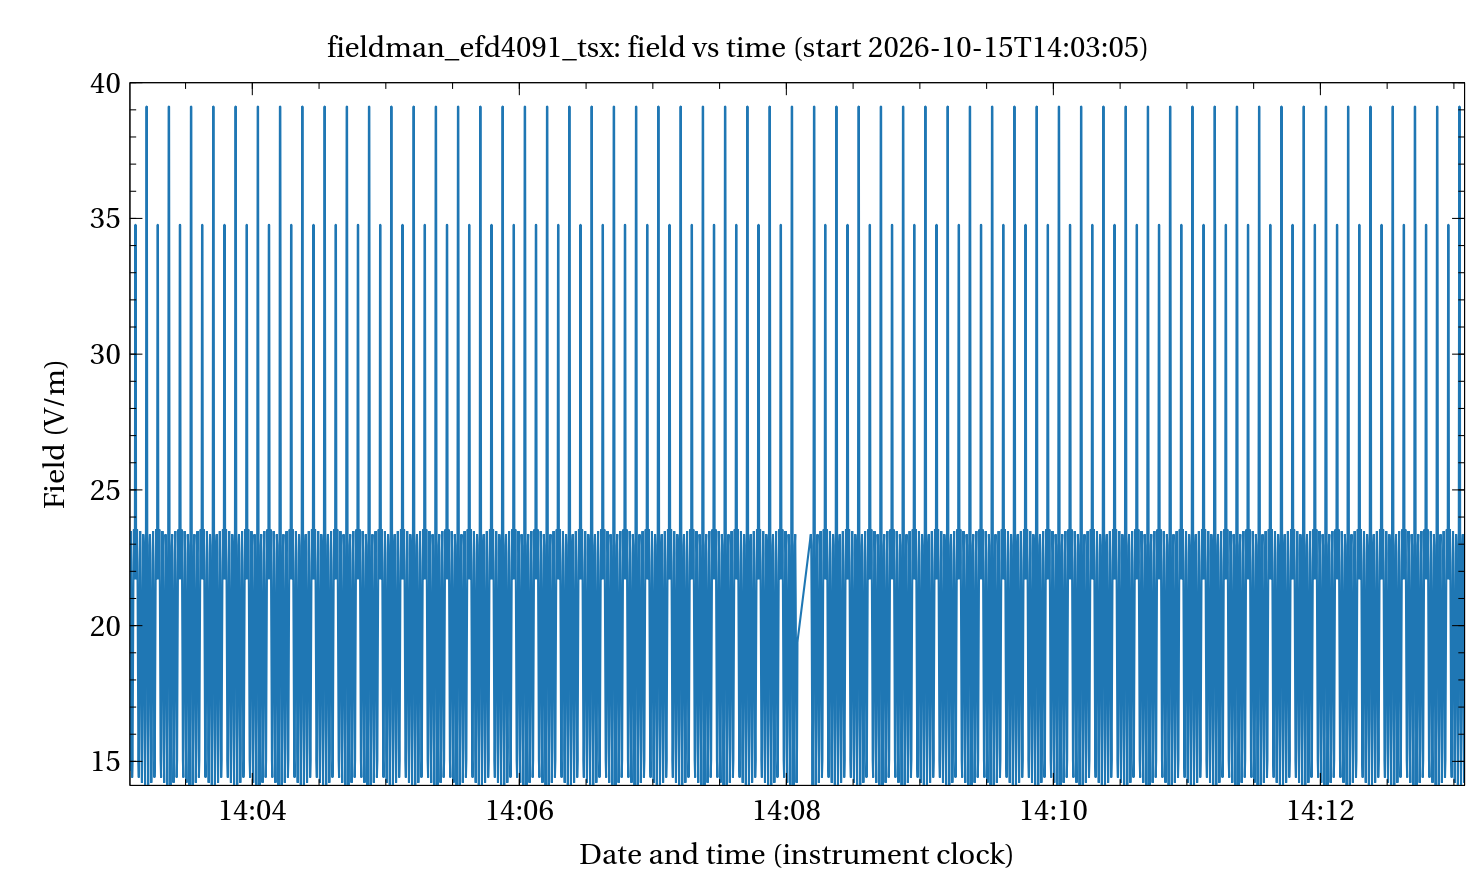
\includegraphics[width=0.92\linewidth]{figures/fig_fieldman_time.png}}{\fbox{\parbox{0.8\linewidth}{\centering Figure file \path{figures/fig_fieldman_time.png} not found: run \path{tools/build_manual_pdf.py --figures}.}}}
\caption{Synthetic FieldMan/Narda-TSX log (EFD-4091): field against the instrument clock on a date axis. The 6\,s gap at 300\,s is deliberate. \emph{(Synthetic data.)}}\label{fig:time}
\end{figure}

\begin{figure}[htbp]
\centering
\IfFileExists{figures/fig_fieldman_amplitude.png}{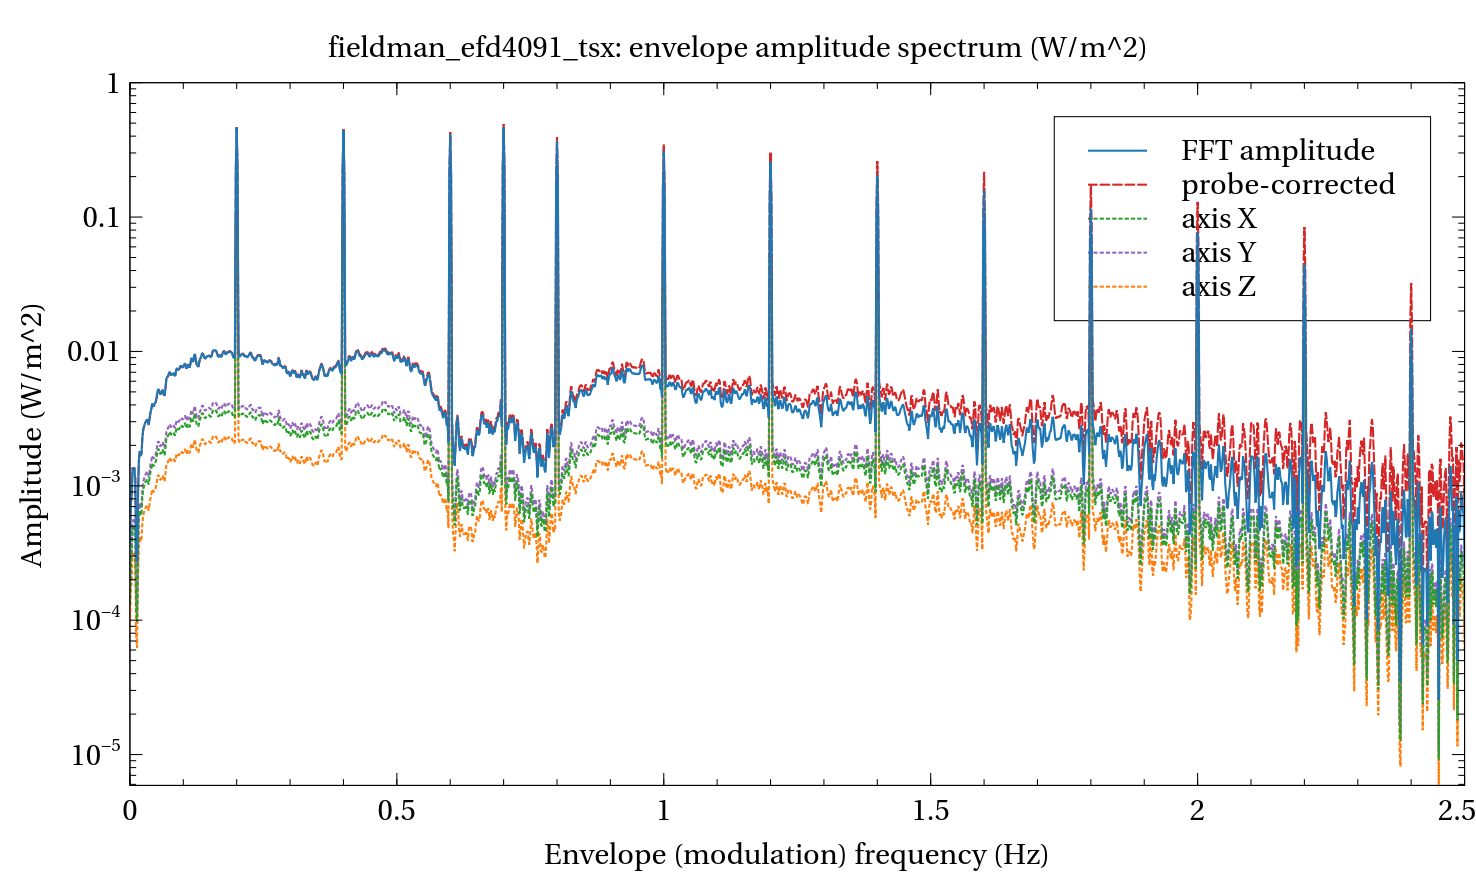
\includegraphics[width=0.92\linewidth]{figures/fig_fieldman_amplitude.png}}{\fbox{\parbox{0.8\linewidth}{\centering Figure file \path{figures/fig_fieldman_amplitude.png} not found: run \path{tools/build_manual_pdf.py --figures}.}}}
\caption{Envelope amplitude spectrum of the same log: the 12\,rpm radar family (0.2\,Hz and harmonics), the 0.7\,Hz source, the probe-corrected trace (dashed) and the X/Y/Z axes (dotted). \emph{(Synthetic data.)}}\label{fig:amplitude}
\end{figure}

\begin{figure}[htbp]
\centering
\IfFileExists{figures/fig_fieldman_zoom.png}{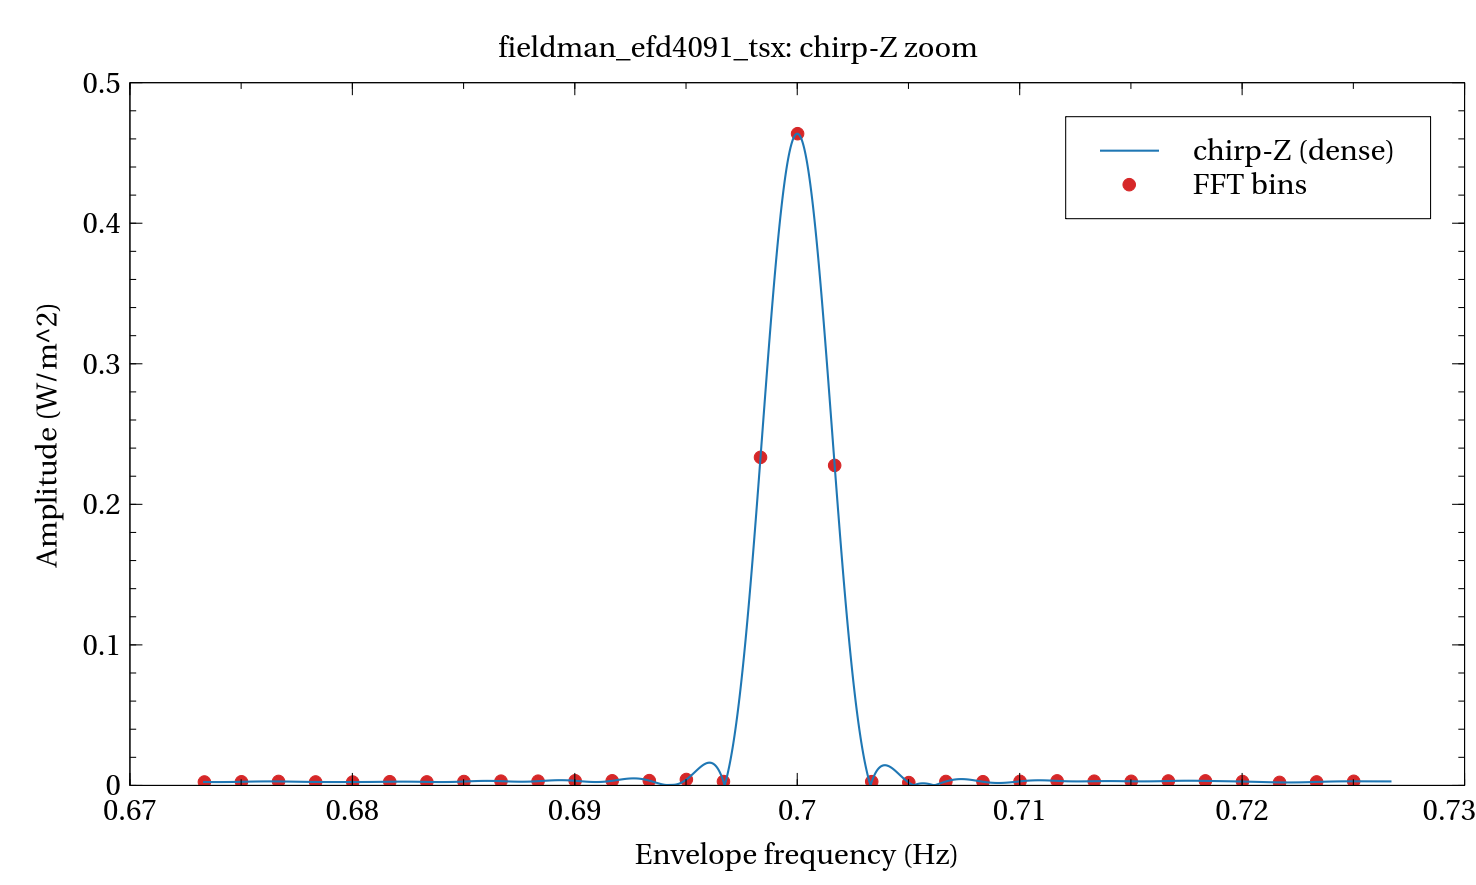
\includegraphics[width=0.92\linewidth]{figures/fig_fieldman_zoom.png}}{\fbox{\parbox{0.8\linewidth}{\centering Figure file \path{figures/fig_fieldman_zoom.png} not found: run \path{tools/build_manual_pdf.py --figures}.}}}
\caption{Chirp-Z zoom around the strongest line: the dense CZT samples (line) between the FFT bins (markers). \emph{(Synthetic data.)}}\label{fig:zoom}
\end{figure}

\begin{figure}[htbp]
\centering
\IfFileExists{figures/fig_fieldman_probe.png}{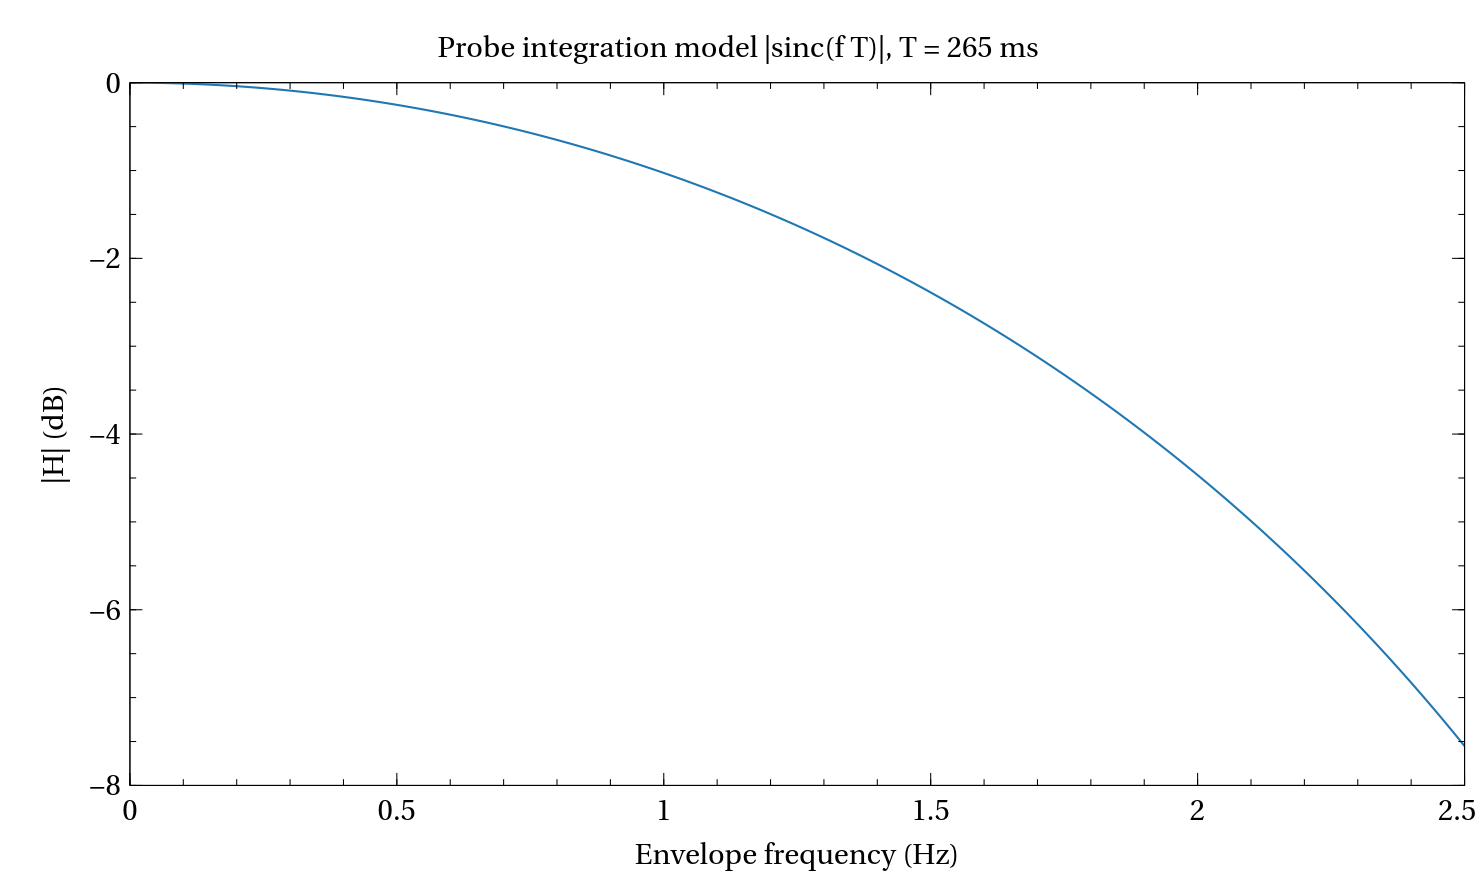
\includegraphics[width=0.92\linewidth]{figures/fig_fieldman_probe.png}}{\fbox{\parbox{0.8\linewidth}{\centering Figure file \path{figures/fig_fieldman_probe.png} not found: run \path{tools/build_manual_pdf.py --figures}.}}}
\caption{Probe integration model $|H(\nu)| = |\operatorname{sinc}(\nu T)|$ for $T = 265$\,ms up to the Nyquist frequency. \emph{(Synthetic data.)}}\label{fig:probe}
\end{figure}

\begin{figure}[htbp]
\centering
\IfFileExists{figures/fig_signalshark_spectrogram.png}{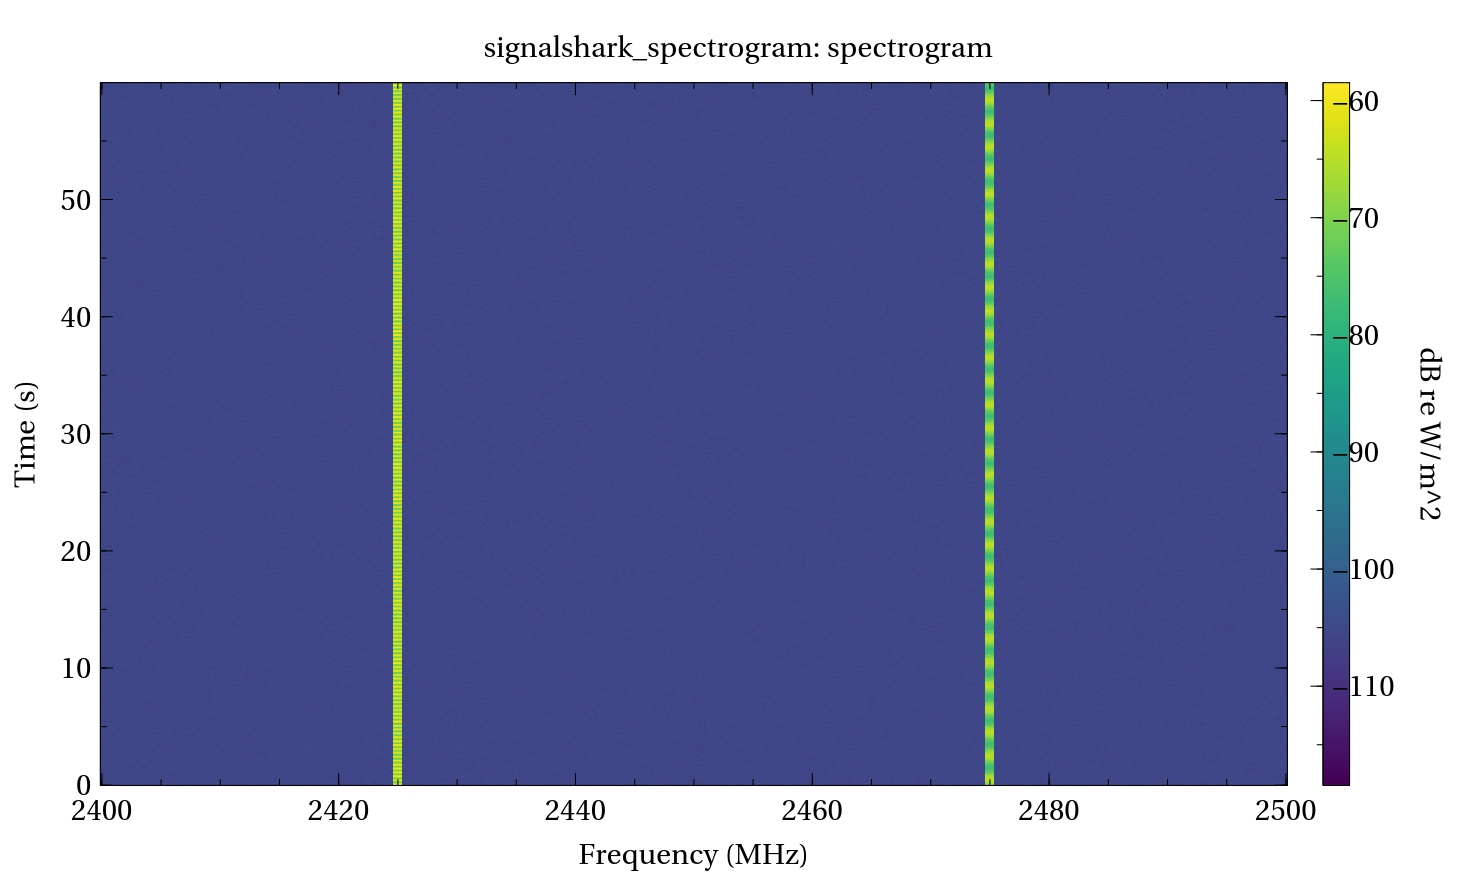
\includegraphics[width=0.92\linewidth]{figures/fig_signalshark_spectrogram.png}}{\fbox{\parbox{0.8\linewidth}{\centering Figure file \path{figures/fig_signalshark_spectrogram.png} not found: run \path{tools/build_manual_pdf.py --figures}.}}}
\caption{Synthetic SignalShark spectrogram: two carriers whose levels vary at 3\,Hz and 0.5\,Hz. \emph{(Synthetic data.)}}\label{fig:spectrogram}
\end{figure}

\begin{figure}[htbp]
\centering
\IfFileExists{figures/fig_signalshark_modulation_map.png}{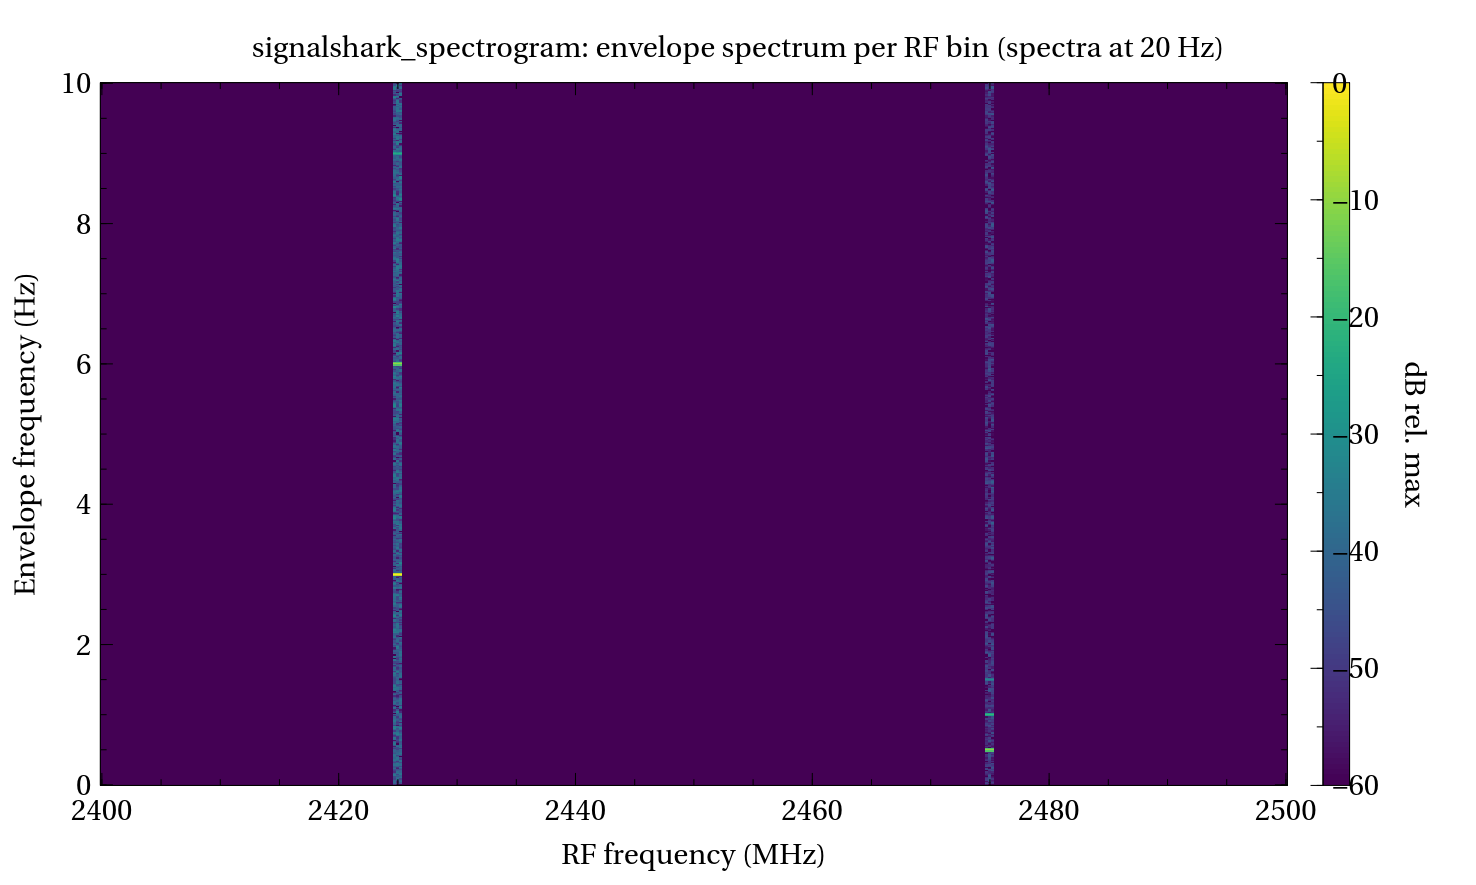
\includegraphics[width=0.92\linewidth]{figures/fig_signalshark_modulation_map.png}}{\fbox{\parbox{0.8\linewidth}{\centering Figure file \path{figures/fig_signalshark_modulation_map.png} not found: run \path{tools/build_manual_pdf.py --figures}.}}}
\caption{Envelope spectrum of every RF bin of that spectrogram: each carrier shows its own modulation frequency. \emph{(Synthetic data.)}}\label{fig:modmap}
\end{figure}

\clearpage

% =============================================================================
%    8  LIVE MODE
% =============================================================================
\section{Live mode}\label{sec:live}
\texttt{--live FILE} follows a text file that another program appends to. New
complete lines are read every \texttt{--update} seconds (default 1\,s; an
unfinished last line waits for the next poll), kept in a ring buffer twice the
size of the analysis window \texttt{--window-s} (default 120\,s), and the
envelope amplitude spectrum and Welch PSD of the latest window are recomputed
and drawn. Every sample is also appended to \path{<file>.live.f64}, raw float64
pairs (time, value) that can be read back with
\verb|np.fromfile(path).reshape(-1, 2)|. \texttt{--no-gui} prints the strongest
lines and families instead; \texttt{--live-seconds} stops after a time.

\begingroup\small
\begin{longtable}{@{}L{\dimexpr 0.12\linewidth-2\tabcolsep\relax}L{\dimexpr 0.3\linewidth-2\tabcolsep\relax}L{\dimexpr 0.54\linewidth-2\tabcolsep\relax}@{}}
\caption{Menus of the live window.}\label{tab:menus}\\
\toprule
\textbf{Menu} & \textbf{Entry} & \textbf{Action} \\
\midrule
\endfirsthead
\multicolumn{3}{@{}l}{\itshape\footnotesize Table \thetable{} (continued)}\\
\toprule
\textbf{Menu} & \textbf{Entry} & \textbf{Action} \\
\midrule
\endhead
\bottomrule
\endlastfoot
File & Save snapshot (.vszh5) & full analysis of the current window; writes the usual output files \\
File & Clear buffer (free RAM) & empties the ring buffer, runs flush\_memory() \\
File & Quit & closes the window \\
View & Light / Dark & palette of the window and plot colours \\
Analysis & Correct probe response & applies -\kern0pt-correct-probe live \\
\end{longtable}
\endgroup


Neither FieldMan nor Narda-TSX documents a continuously written file or a
streaming interface for the broadband probes \cite{R5,R9}, so whether live mode
works with them depends on how they write data; it was tested with a file
written in real time by a script. NBM-550 remote output (\texttt{MEAS\_START},
5, 50 or 60 samples per second \cite{R6}) logged to a file by another tool is a
documented route.

\begin{figure}[htbp]
\centering
\IfFileExists{figures/fig_live_window_dark.png}{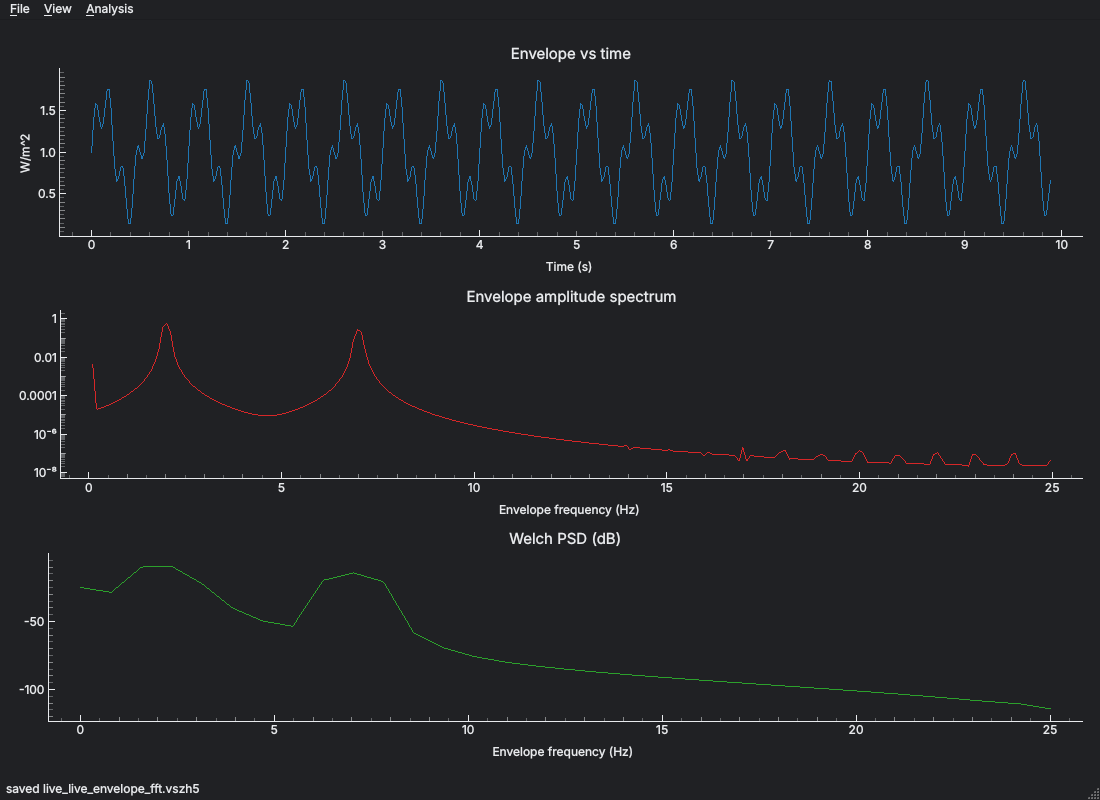
\includegraphics[width=0.92\linewidth]{figures/fig_live_window_dark.png}}{\fbox{\parbox{0.8\linewidth}{\centering Figure file \path{figures/fig_live_window_dark.png} not found: run \path{tools/build_manual_pdf.py --figures}.}}}
\caption{Live window (View $\rightarrow$ Dark) following a growing file with 2\,Hz and 7\,Hz envelope tones. \emph{(Synthetic data.)}}\label{fig:live}
\end{figure}


% =============================================================================
%    9  MEMORY, PARALLEL PROCESSING AND GPU
% =============================================================================
\section{Memory, parallel processing and GPU}\label{sec:memory}
\begin{itemize}
\item \textbf{Spill to disk}: a column longer than 20\,000\,000 samples is moved
from RAM to a temporary raw file and used as a memory map; the files are
deleted when the program exits. A 2.4-million-row, 900\,Hz test log was
analysed this way.
\item \textbf{Chunks and batches}: text files are read 500\,000 rows at a time;
Welch processes 512 segments at a time; Lomb--Scargle about 64\,MiB of
frequencies at a time; the per-bin modulation spectra in batches of about
256\,MiB.
\item \textbf{Freeing memory}: \texttt{flush\_memory()} runs the garbage
collector and empties the CuPy memory pools; batch mode calls it after each
file, and the live window's \emph{File $\rightarrow$ Clear buffer} too.
\texttt{--pickle} also writes the whole result object to
\path{<stem>_result.pkl} (load it with \texttt{load\_pickle}, only from files you
trust).
\item \textbf{Parallel}: \texttt{--jobs N} analyses N files in separate processes;
each process then uses one FFT thread so that the cores are not
oversubscribed. With one job, SciPy's FFTs use every core.
\item \textbf{GPU}: \texttt{--gpu} moves the FFTs, Welch segments, modulation
spectra and Lomb--Scargle sums to an NVIDIA GPU through CuPy \cite{B27}. Without
CuPy or a CUDA device the program continues on the CPU and says why in the
summary (\texttt{backend}).
\end{itemize}

% =============================================================================
%    10  WORKING IN SPYDER
% =============================================================================
\section{Working in Spyder}\label{sec:spyder}
The script is organised in Spyder cells, each opened by a banner
\verb|# %% ====| and a title line. Table~\ref{tab:cells} lists them with the
functions and classes each defines (generated from the script). Run the cells
from the top; the last cell is a commented scratch cell:
\begin{Verbatim}
opts = Options(probe="EFD-4091", correct_probe=True, lomb="on")
print(inspect_input(r"C:\path\to\export.csv", opts))
series = load_any(r"C:\path\to\export.csv", opts)
result = analyse_timeseries(series, opts)
print(result.peaks[:5], result.families)
write_outputs(result, Path(r"C:\path\to\out"), opts)
flush_memory()
\end{Verbatim}

\begingroup\footnotesize
\begin{longtable}{@{}L{\dimexpr 0.06\linewidth-2\tabcolsep\relax}L{\dimexpr 0.27\linewidth-2\tabcolsep\relax}L{\dimexpr 0.07\linewidth-2\tabcolsep\relax}L{\dimexpr 0.58\linewidth-2\tabcolsep\relax}@{}}
\caption{Spyder cells of emf\_envelope\_fft\_v0\_0\_2.py.}\label{tab:cells}\\
\toprule
\textbf{No.} & \textbf{Cell} & \textbf{Line} & \textbf{Definitions} \\
\midrule
\endfirsthead
\multicolumn{4}{@{}l}{\itshape\footnotesize Table \thetable{} (continued)}\\
\toprule
\textbf{No.} & \textbf{Cell} & \textbf{Line} & \textbf{Definitions} \\
\midrule
\endhead
\bottomrule
\endlastfoot
1 & MODULE HEADER & 6 & \textit{(constants, imports or comments)} \\
2 & IMPORTS & 232 & \textit{(constants, imports or comments)} \\
3 & CONSTANTS, PROBE CATALOGUE AND UNITS & 295 & ProbeSpec, lookup\_probe, parse\_unit, to\_power\_like, to\_field\_like \\
4 & DATA MODEL & 486 & TimeSeries, SpectrumSet, Options \\
5 & MEMORY HELPERS (bounded RAM for long logs) & 582 & \_remove\_spill\_files, SpillBuffer, flush\_memory, save\_pickle, load\_pickle \\
6 & COMPUTE BACKEND (CPU / optional GPU) & 695 & Backend \\
7 & TEXT EXPORT SNIFFING AND READING & 736 & TextLayout, \_read\_head, \_is\_number, \_split, sniff\_text, \_pick\_columns, TimeOrigin, \_to\_seconds, \_origin\_text, ... (23 in all) \\
8 & PRE-PROCESSING: TIMING, GAPS, UNIFORM GRID & 1409 & UniformSeries, make\_uniform, analysis\_quantity \\
9 & SPECTRAL ESTIMATORS & 1491 & amplitude\_spectrum, welch\_blocks, czt\_zoom, lomb\_scargle, envelope\_spectrogram, probe\_response, correct\_probe \\
10 & PEAKS AND HARMONIC FAMILIES & 1635 & find\_spectral\_peaks, harmonic\_families \\
11 & ANALYSIS DRIVERS & 1702 & SeriesResult, \_default\_nperseg, analyse\_timeseries, SpectrogramResult, \_decimate\_max, analyse\_spectrumset \\
12 & VEUSZ .vszh5 OUTPUT (through the author's vszh5\_writer.py) & 2028 & \_freq\_unit, bookmark\_outline, \_write\_series\_pages, write\_vszh5\_series, write\_vszh5\_spectrogram \\
13 & OTHER OUTPUTS: CSV, NPZ, JSON SUMMARY, OPTIONAL RENDER & 2249 & \_summary\_series, \_summary\_spectrogram, \_jsonable, \_write\_csv, write\_outputs, render\_vszh5 \\
14 & BATCH (PARALLEL) PROCESSING & 2364 & process\_file, process\_files \\
15 & LIVE MODE: FOLLOW A GROWING FILE & 2411 & LiveTail, RingBuffer, live\_update, \_live\_ring, run\_live\_console, run\_live\_gui \\
16 & SELF-TEST WITH SYNTHETIC EXPORTS & 2743 & \_synthetic\_radar, \_probe\_filter, make\_synthetic\_files, self\_test \\
17 & COMMAND LINE & 2922 & build\_parser, options\_from\_args, main \\
18 & INTERACTIVE SCRATCH CELL (Spyder) & 3022 & \textit{(constants, imports or comments)} \\
\end{longtable}
\endgroup


% =============================================================================
%    11  VERIFICATION
% =============================================================================
\section{Verification}\label{sec:verification}
\texttt{--selftest} checks the estimators against known answers and then runs
every reader on synthetic files written in the styles expected from the
instruments (semicolon and decimal comma with German dates, a 1\,s NBM timer
log, an EHP-50 TS folder, a SignalShark-like HDF5 file and a converter CSV).
Table~\ref{tab:selftest} is the result of the run made while building this
manual.

\begingroup\footnotesize
\begin{longtable}{@{}L{\dimexpr 0.42\linewidth-2\tabcolsep\relax}L{\dimexpr 0.42\linewidth-2\tabcolsep\relax}L{\dimexpr 0.1\linewidth-2\tabcolsep\relax}@{}}
\caption{Self-test result (program 0.0.2, run during this build).}\label{tab:selftest}\\
\toprule
\textbf{Check} & \textbf{Measured} & \textbf{Result} \\
\midrule
\endfirsthead
\multicolumn{3}{@{}l}{\itshape\footnotesize Table \thetable{} (continued)}\\
\toprule
\textbf{Check} & \textbf{Measured} & \textbf{Result} \\
\midrule
\endhead
\bottomrule
\endlastfoot
streamed Welch == scipy.signal.welch & max rel err 3.6e-15 & PASS \\
FFT amplitude of 0.8 sinusoid & 0.802 & PASS \\
CZT peak frequency & 0.21000 Hz & PASS \\
Lomb-Scargle amplitude and frequency & 0.799 at 0.2100 Hz & PASS \\
|sinc| at 1.5 Hz, T=265 ms & -2.39 dB & PASS \\
FieldMan/TSX & radar 12 rpm family: [12.0, 42.0] & PASS \\
FieldMan/TSX & 0.7 Hz source found & PASS \\
NBM timer log & 6 rpm: [6.0] & PASS \\
EHP-50 TS spectra folder & 0.05 Hz modulation of 50 Hz line: [0.05, 0.05] & PASS \\
signalshark & per-channel envelope 0.5 and 3 Hz: [0.5, 3.0] & PASS \\
signalshark\_csv & per-channel envelope 0.5 and 3 Hz: [0.5, 3.0] & PASS \\
.vszh5 layout (Veusz format 1) & signalshark\_converted\_envelope\_fft.vszh5 & PASS \\
\end{longtable}
\endgroup


Further checks made for version 0.0.2:
\begin{itemize}
\item Every summary and CSV of the self-test compared with version 0.0.1: all
numbers identical (two summary keys of the spectrogram result were renamed,
see Appendix~\ref{app:history}).
\item Rendering in Veusz 4.2.1 of a probe log (6 pages) and a SignalShark
spectrogram (16 pages): date axis, line styles, markers, colour bars and the
bookmark tree checked by eye and with pypdf.
\item Live mode, console and window (light and dark), following a file written
at 50 samples per second with 2\,Hz and 7\,Hz tones: both found; snapshot saved.
\item A 2.4-million-row 900\,Hz log through the spill-to-disk path: lines at
37.0 and 120.0\,Hz found exactly.
\item Three files with \texttt{--jobs 3 --gpu} on a machine without CuPy: all
analysed, CPU fallback reported.
\end{itemize}

% =============================================================================
%    12  LIMITATIONS AND KNOWN ISSUES
% =============================================================================
\section{Limitations and known issues}\label{sec:limits}
\begin{enumerate}
\item The readers are heuristic until real exports of FieldMan, Narda-TSX,
NBM-TS, EHP-50 TS and SignalShark have been examined; use \texttt{--inspect}.
\item ``EFD-4091E'' is treated as the EFD-4091; no datasheet for an E variant
was found.
\item The probe averaging is modelled as a boxcar of the nominal integration
time; the EF\,0691's integration time is not published, so $1/f_s$ is assumed.
\item The probe correction switches from the exact inverse to the Wiener-type
gain at $|H| = 1/g_\mathrm{max}$ with a step of 1.94\,dB
(Section~\ref{sec:correction}); it matters only for probes whose first null lies
below their Nyquist frequency. A smooth transition is planned.
\item Content above the Nyquist frequency aliases; nothing in the data can
remove it after the fact.
\item Above the True-RMS range the diodes leave square-law operation and powers
no longer add; the envelope spectrum is then distorted (a warning is given).
\item The time page plots every sample, so very long logs make large PDFs.
\item Live mode depends on how the instrument software writes its files
(Section~\ref{sec:live}).
\end{enumerate}

% =============================================================================
%    13  TROUBLESHOOTING
% =============================================================================
\section{Troubleshooting}\label{sec:troubleshooting}

\begingroup\small
\begin{longtable}{@{}L{\dimexpr 0.3\linewidth-2\tabcolsep\relax}L{\dimexpr 0.32\linewidth-2\tabcolsep\relax}L{\dimexpr 0.34\linewidth-2\tabcolsep\relax}@{}}
\caption{Troubleshooting.}\label{tab:trouble}\\
\toprule
\textbf{Symptom} & \textbf{Likely cause} & \textbf{Remedy} \\
\midrule
\endfirsthead
\multicolumn{3}{@{}l}{\itshape\footnotesize Table \thetable{} (continued)}\\
\toprule
\textbf{Symptom} & \textbf{Likely cause} & \textbf{Remedy} \\
\midrule
\endhead
\bottomrule
\endlastfoot
'no value column found' & unusual column names & -\kern0pt-value-col NAME (or index) \\
time axis wrong or 'cannot parse' & unusual date format, month/day order & -\kern0pt-time-col, -\kern0pt-dayfirst; check with -\kern0pt-inspect \\
numbers 1000x too large & decimal comma read as thousands & -\kern0pt-decimal , -\kern0pt-sep ; \\
'measured sample rate differs' & logging interval longer than the probe rate & expected with timer logs; Nyquist is then lower \\
lines at 2f, f1+f2 & -\kern0pt-quantity field & use the default -\kern0pt-quantity power \\
SignalShark axes look wrong & unknown .h5 layout & -\kern0pt-inspect, then -\kern0pt-h5-level/-\kern0pt-h5-freq/-\kern0pt-h5-time \\
dBm levels, no W/m\textasciicircum{}2 & no antenna factor & -\kern0pt-antenna-factor-db AF \\
-\kern0pt-render: 'Veusz not found' & Veusz not on PATH & set VEUSZ\_EXE to veusz.exe; the .vszh5 is written anyway \\
ImportError: vszh5\_writer too old & an older copy imported first (Spyder) & restart the kernel; keep 0.0.11 next to the script \\
-\kern0pt-gpu but 'CPU' in backend & no CuPy or CUDA device & mamba install -c conda-forge cupy; NVIDIA only \\
live: 'waiting for data' & file has no complete row yet, or other layout & check the file grows; -\kern0pt-inspect it once \\
\end{longtable}
\endgroup


% =============================================================================
%    APPENDIX A  PYTHON MODULES USED
% =============================================================================
\clearpage
\appendix
\section{Python modules used}\label{app:modules}
This appendix lists every Python module the analyzer uses, the functions,
classes and methods it calls, how it calls them and why that module was
chosen. Table~\ref{tab:modules} is the overview; the following subsections
give the details, module by module. Versions are those of the tested
environment (2026-10-15).

\begingroup\small
\begin{longtable}{@{}L{\dimexpr 0.17\linewidth-2\tabcolsep\relax}L{\dimexpr 0.1\linewidth-2\tabcolsep\relax}L{\dimexpr 0.3\linewidth-2\tabcolsep\relax}L{\dimexpr 0.39\linewidth-2\tabcolsep\relax}@{}}
\caption{Python modules used by the analyzer.}\label{tab:modules}\\
\toprule
\textbf{Module} & \textbf{Tested} & \textbf{Needed for} & \textbf{Why this module} \\
\midrule
\endfirsthead
\multicolumn{4}{@{}l}{\itshape\footnotesize Table \thetable{} (continued)}\\
\toprule
\textbf{Module} & \textbf{Tested} & \textbf{Needed for} & \textbf{Why this module} \\
\midrule
\endhead
\bottomrule
\endlastfoot
\texttt{numpy} & 2.5.4 & all arrays and array maths & common array type of every library used \\
\texttt{scipy} & 1.18.1 & FFT, windows, CZT, short-time FFT, peaks, interpolation & tested implementations of every estimator needed; scikit-rf has none of them \\
\texttt{pandas} & 3.0.6 & reading text and Excel exports & fast chunked CSV reader, tolerant date parsing \\
\texttt{openpyxl} & 3.1.5 & .xlsx (engine of pandas) & pandas' reader for .xlsx \\
\texttt{h5py} & 3.16.0 & SignalShark .h5; .vszh5 output & direct HDF5 access incl. references \\
\texttt{vszh5\_writer} & 0.0.11 & Veusz documents, rendering & the author's Veusz writer \\
\texttt{Qt.py + PySide6} & 2.0.7 / 6.12 & live window & one Qt API, PySide6 binding \\
\texttt{pyqtgraph} & 0.14.0 & live plots & fast repeated plot updates \\
\texttt{cupy} & optional & -\kern0pt-gpu & NumPy interface on NVIDIA GPUs \\
\texttt{pypdf} & 6.20.1 & PDF bookmarks (-\kern0pt-render, manual check) & pure Python PDF editing \\
\texttt{veusz} & 4.2.1 & rendering (-\kern0pt-render) & the plotting program of the documents \\
standard library & 3.12.13 & CLI, files, processes, time, JSON, ... & no extra dependency \\
\end{longtable}
\endgroup


\subsection{NumPy}\label{app:numpy}
NumPy \cite{B20} holds every array of the program. It was chosen because SciPy,
pandas, h5py, CuPy and pyqtgraph all exchange data as NumPy arrays, so no
conversion is needed anywhere.

\begingroup\footnotesize
\begin{longtable}{@{}L{\dimexpr 0.26\linewidth-2\tabcolsep\relax}L{\dimexpr 0.22\linewidth-2\tabcolsep\relax}L{\dimexpr 0.48\linewidth-2\tabcolsep\relax}@{}}
\caption{NumPy calls.}\label{tab:numpy}\\
\toprule
\textbf{Call} & \textbf{Where (function)} & \textbf{How and why} \\
\midrule
\endfirsthead
\multicolumn{3}{@{}l}{\itshape\footnotesize Table \thetable{} (continued)}\\
\toprule
\textbf{Call} & \textbf{Where (function)} & \textbf{How and why} \\
\midrule
\endhead
\bottomrule
\endlastfoot
\texttt{np.\allowbreak{}asarray,\allowbreak{} np.\allowbreak{}ascontiguousarray} & everywhere & convert inputs to float64; contiguous arrays for FFTs and HDF5 writes \\
\texttt{np.\allowbreak{}argsort(\allowbreak{}kind=\allowbreak{}'stable'),\allowbreak{} np.\allowbreak{}unique} & make\_\allowbreak{}uniform, read\_\allowbreak{}signalshark\_\allowbreak{}csv & sort time stamps keeping equal stamps in order, drop duplicates; pivot long-format CSV \\
\texttt{np.\allowbreak{}diff,\allowbreak{} np.\allowbreak{}median,\allowbreak{} ndarray.\allowbreak{}mean} & make\_\allowbreak{}uniform, analyse\_\allowbreak{}spectrumset & sample interval = mean of gap-free intervals; jitter = median deviation \\
\texttt{np.\allowbreak{}interp} & make\_\allowbreak{}uniform, read\_\allowbreak{}ehp\_\allowbreak{}folder & linear interpolation onto the uniform grid / common frequency axis: local, no overshoot, O(N) \\
\texttt{np.\allowbreak{}memmap,\allowbreak{} ndarray.\allowbreak{}tofile} & SpillBuffer, RingBuffer & long columns live in a raw file mapped into memory, so RAM stays bounded; live log on disk \\
\texttt{np.\allowbreak{}sinc} & probe\_\allowbreak{}response & normalised sinc sin(pi x)/(pi x), the boxcar response of eq. (sinc) \\
\texttt{np.\allowbreak{}log10,\allowbreak{} np.\allowbreak{}maximum} & all dB conversions & dB values with a floor, so log10(0) never occurs \\
\texttt{np.\allowbreak{}nanmean,\allowbreak{} np.\allowbreak{}nanmax,\allowbreak{} np.\allowbreak{}nansum,\allowbreak{} np.\allowbreak{}where} & analyse\_\allowbreak{}spectrumset & spectrogram statistics with missing cells (NaN) ignored \\
\texttt{np.\allowbreak{}stack,\allowbreak{} np.\allowbreak{}column\_\allowbreak{}stack,\allowbreak{} np.\allowbreak{}vstack} & welch\_\allowbreak{}blocks, readers, outputs & batch of Welch segments; tables for CSV; spectra of an EHP folder \\
\texttt{np.\allowbreak{}linspace,\allowbreak{} np.\allowbreak{}arange} & czt\_\allowbreak{}zoom, lomb\_\allowbreak{}scargle, synthetic files & frequency grids and time axes \\
\texttt{np.\allowbreak{}convolve} & \_\allowbreak{}probe\_\allowbreak{}filter (self-test) & boxcar-average synthetic data like a probe \\
\texttt{np.\allowbreak{}savetxt,\allowbreak{} np.\allowbreak{}savez\_\allowbreak{}compressed} & \_\allowbreak{}write\_\allowbreak{}csv, write\_\allowbreak{}outputs & CSV and compressed .npz outputs \\
\texttt{np.\allowbreak{}random.\allowbreak{}default\_\allowbreak{}rng} & self-test & reproducible synthetic noise and jitter \\
\end{longtable}
\endgroup


\subsection{SciPy}\label{app:scipy}
SciPy \cite{R10} supplies the spectral estimators. It provides, in one tested
library, everything the problem needs: real FFTs with multithreading, standard
windows, the chirp-Z zoom, the short-time FFT and peak finding. scikit-rf
\cite{R15} was considered and not used: it is built for network parameters
(S-parameters, Touchstone files, calibration), not for spectral analysis of time
series.

\begingroup\footnotesize
\begin{longtable}{@{}L{\dimexpr 0.26\linewidth-2\tabcolsep\relax}L{\dimexpr 0.22\linewidth-2\tabcolsep\relax}L{\dimexpr 0.48\linewidth-2\tabcolsep\relax}@{}}
\caption{SciPy calls.}\label{tab:scipy}\\
\toprule
\textbf{Call} & \textbf{Where (function)} & \textbf{How and why} \\
\midrule
\endfirsthead
\multicolumn{3}{@{}l}{\itshape\footnotesize Table \thetable{} (continued)}\\
\toprule
\textbf{Call} & \textbf{Where (function)} & \textbf{How and why} \\
\midrule
\endhead
\bottomrule
\endlastfoot
\texttt{scipy.\allowbreak{}fft.\allowbreak{}rfft(\allowbreak{}x,\allowbreak{} n,\allowbreak{} axis,\allowbreak{} workers)} & amplitude\_\allowbreak{}spectrum, welch\_\allowbreak{}blocks, analyse\_\allowbreak{}spectrumset & FFT of real data (half the work of a complex FFT); workers = threads (-1 all, 1 per process in batch mode) \\
\texttt{scipy.\allowbreak{}fft.\allowbreak{}rfftfreq(\allowbreak{}n,\allowbreak{} d)} & same & frequency of every rfft bin \\
\texttt{scipy.\allowbreak{}signal.\allowbreak{}get\_\allowbreak{}window(\allowbreak{}name,\allowbreak{} N)} & every estimator & any SciPy window by name (-\kern0pt-window); periodic form (fftbins=True), correct for spectral analysis \\
\texttt{scipy.\allowbreak{}signal.\allowbreak{}zoom\_\allowbreak{}fft(\allowbreak{}x,\allowbreak{} [f1,\allowbreak{} f2],\allowbreak{} m,\allowbreak{} fs,\allowbreak{} endpoint=\allowbreak{}True)} & czt\_\allowbreak{}zoom & chirp-Z zoom (Bluestein), dense spectrum samples in a band \\
\texttt{scipy.\allowbreak{}signal.\allowbreak{}ShortTimeFFT(\allowbreak{}win,\allowbreak{} hop,\allowbreak{} fs,\allowbreak{} fft\_\allowbreak{}mode=\allowbreak{}'onesided2X',\allowbreak{} scale\_\allowbreak{}to=\allowbreak{}'psd')} & envelope\_\allowbreak{}spectrogram & spectrogram(detr='constant', p0, p1), lower\_border\_end, upper\_border\_begin, t(), f: one-sided PSD slices without the slices hanging over the ends (SciPy >= 1.12) \\
\texttt{scipy.\allowbreak{}signal.\allowbreak{}find\_\allowbreak{}peaks(\allowbreak{}x,\allowbreak{} height,\allowbreak{} prominence)} & find\_\allowbreak{}spectral\_\allowbreak{}peaks, analyse\_\allowbreak{}spectrumset & local maxima above a level and prominence: envelope lines; carriers for channels \\
\texttt{scipy.\allowbreak{}signal.\allowbreak{}welch(\allowbreak{}.\allowbreak{}.\allowbreak{}.\allowbreak{})} & self\_\allowbreak{}test only & reference to which welch\_blocks is compared \\
\texttt{scipy.\allowbreak{}interpolate.\allowbreak{}interp1d(\allowbreak{}x,\allowbreak{} y,\allowbreak{} axis=\allowbreak{}0)} & analyse\_\allowbreak{}spectrumset & all frequency bins of a spectrogram onto a uniform time grid in one call (a legacy SciPy class, still supported) \\
\end{longtable}
\endgroup


\subsection{pandas and openpyxl}\label{app:pandas}
pandas \cite{B21} reads the text and Excel exports. Its CSV reader is fast (C
engine), reads in chunks, and its date parser copes with the many date and time
formats instrument software writes \cite{B33}. openpyxl \cite{B34} is not imported by the
program; pandas uses it as the engine for \texttt{.xlsx} files.

\begingroup\footnotesize
\begin{longtable}{@{}L{\dimexpr 0.26\linewidth-2\tabcolsep\relax}L{\dimexpr 0.22\linewidth-2\tabcolsep\relax}L{\dimexpr 0.48\linewidth-2\tabcolsep\relax}@{}}
\caption{pandas calls.}\label{tab:pandas}\\
\toprule
\textbf{Call} & \textbf{Where (function)} & \textbf{How and why} \\
\midrule
\endfirsthead
\multicolumn{3}{@{}l}{\itshape\footnotesize Table \thetable{} (continued)}\\
\toprule
\textbf{Call} & \textbf{Where (function)} & \textbf{How and why} \\
\midrule
\endhead
\bottomrule
\endlastfoot
\texttt{pd.\allowbreak{}read\_\allowbreak{}csv(\allowbreak{}sep,\allowbreak{} decimal,\allowbreak{} encoding,\allowbreak{} skiprows,\allowbreak{} header=\allowbreak{}None,\allowbreak{} usecols,\allowbreak{} dtype=\allowbreak{}str,\allowbreak{} chunksize,\allowbreak{} engine,\allowbreak{} on\_\allowbreak{}bad\_\allowbreak{}lines=\allowbreak{}'skip')} & read\_\allowbreak{}text\_\allowbreak{}timeseries, read\_\allowbreak{}text\_\allowbreak{}spectrum, read\_\allowbreak{}signalshark\_\allowbreak{}csv & reads only the needed columns as text, in chunks (bounded memory); bad lines skipped; numbers converted afterwards so decimal commas and thousands dots are handled \\
\texttt{Series.\allowbreak{}str.\allowbreak{}strip/\allowbreak{}.\allowbreak{}replace/\allowbreak{}.\allowbreak{}match} & \_\allowbreak{}num, \_\allowbreak{}to\_\allowbreak{}seconds & clean quotes and spaces; decimal comma \\
\texttt{pd.\allowbreak{}to\_\allowbreak{}numeric(\allowbreak{}errors=\allowbreak{}'coerce')} & \_\allowbreak{}num, \_\allowbreak{}to\_\allowbreak{}seconds & text to numbers, NaN where not a number \\
\texttt{pd.\allowbreak{}to\_\allowbreak{}datetime(\allowbreak{}format=\allowbreak{}'mixed',\allowbreak{} dayfirst,\allowbreak{} errors=\allowbreak{}'coerce')} & \_\allowbreak{}to\_\allowbreak{}seconds, LiveTail.\allowbreak{}poll & date/time strings of any common format; .dt.tz\_convert(None), .dt.total\_seconds() give seconds \\
\texttt{pd.\allowbreak{}read\_\allowbreak{}excel(\allowbreak{}sheet\_\allowbreak{}name=\allowbreak{}0,\allowbreak{} header=\allowbreak{}None,\allowbreak{} dtype=\allowbreak{}str)} & read\_\allowbreak{}xlsx\_\allowbreak{}timeseries & first sheet as text (openpyxl engine), then the CSV reader path \\
\texttt{DataFrame.\allowbreak{}to\_\allowbreak{}csv(\allowbreak{}sep=\allowbreak{}';')} & read\_\allowbreak{}xlsx\_\allowbreak{}timeseries & temporary CSV of the sheet \\
\end{longtable}
\endgroup


\subsection{h5py}\label{app:h5py}
h5py \cite{B22} reads SignalShark \texttt{.h5} files and, through
\path{vszh5_writer.py}, writes the Veusz \texttt{.vszh5} documents, which are
HDF5 files. It gives direct access to groups, datasets, attributes and object
references, which the Veusz format needs.

\begingroup\footnotesize
\begin{longtable}{@{}L{\dimexpr 0.26\linewidth-2\tabcolsep\relax}L{\dimexpr 0.22\linewidth-2\tabcolsep\relax}L{\dimexpr 0.48\linewidth-2\tabcolsep\relax}@{}}
\caption{h5py calls.}\label{tab:h5py}\\
\toprule
\textbf{Call} & \textbf{Where (function)} & \textbf{How and why} \\
\midrule
\endfirsthead
\multicolumn{3}{@{}l}{\itshape\footnotesize Table \thetable{} (continued)}\\
\toprule
\textbf{Call} & \textbf{Where (function)} & \textbf{How and why} \\
\midrule
\endhead
\bottomrule
\endlastfoot
\texttt{h5py.\allowbreak{}File(\allowbreak{}path,\allowbreak{} 'r')} & read\_\allowbreak{}signalshark\_\allowbreak{}h5, describe\_\allowbreak{}h5, self\_\allowbreak{}test & open HDF5 read-only \\
\texttt{File.\allowbreak{}visititems(\allowbreak{}callback)} & read\_\allowbreak{}signalshark\_\allowbreak{}h5, describe\_\allowbreak{}h5 & walk every group and dataset to find level and axis datasets / print the tree \\
\texttt{Dataset.\allowbreak{}ndim/\allowbreak{}.\allowbreak{}shape/\allowbreak{}.\allowbreak{}dtype,\allowbreak{} .\allowbreak{}attrs,\allowbreak{} .\allowbreak{}parent} & read\_\allowbreak{}signalshark\_\allowbreak{}h5 & choose datasets by shape and type; gather attributes up to the root (units, start/stop) \\
\texttt{h5py.\allowbreak{}File(\allowbreak{}path,\allowbreak{} 'w'),\allowbreak{} create\_\allowbreak{}group,\allowbreak{} create\_\allowbreak{}dataset(\allowbreak{}compression=\allowbreak{}'gzip',\allowbreak{} compression\_\allowbreak{}opts=\allowbreak{}4,\allowbreak{} shuffle=\allowbreak{}True)} & vszh5\_\allowbreak{}writer.\allowbreak{}VeuszWriter & the .vszh5 layout, gzip for arrays of 4096+ values \\
\texttt{Dataset.\allowbreak{}ref (\allowbreak{}object reference)} & vszh5\_\allowbreak{}writer.\allowbreak{}VeuszWriter.\allowbreak{}dataset\_\allowbreak{}2d & links an image to its axis arrays (vsz\_xrange etc.), as Veusz itself does \\
\end{longtable}
\endgroup


\subsection{vszh5\_writer (the author's module, 0.0.11)}\label{app:writer}
\path{vszh5_writer.py} writes Veusz's native HDF5 document format without
Veusz, and renders it to PDF and PNG when Veusz is installed. It came from the
author's \path{isp_speed_monitor.py} and the QuickSyn package (0.0.10); for this
program it was extended to 0.0.11 with two-dimensional datasets and plot-page
helpers, without changing any existing call; the 2-D layout follows the Veusz source \cite{B29}. The analyzer uses it for every
Veusz document, so the pages look the same as in the author's other programs.

\begingroup\footnotesize
\begin{longtable}{@{}L{\dimexpr 0.26\linewidth-2\tabcolsep\relax}L{\dimexpr 0.22\linewidth-2\tabcolsep\relax}L{\dimexpr 0.48\linewidth-2\tabcolsep\relax}@{}}
\caption{vszh5\_writer calls.}\label{tab:writer}\\
\toprule
\textbf{Call} & \textbf{Where (function)} & \textbf{How and why} \\
\midrule
\endfirsthead
\multicolumn{3}{@{}l}{\itshape\footnotesize Table \thetable{} (continued)}\\
\toprule
\textbf{Call} & \textbf{Where (function)} & \textbf{How and why} \\
\midrule
\endhead
\bottomrule
\endlastfoot
\texttt{VeuszWriter(\allowbreak{}path,\allowbreak{} compress=\allowbreak{}True,\allowbreak{} writer\_\allowbreak{}tag)} & write\_\allowbreak{}vszh5\_\allowbreak{}series, write\_\allowbreak{}vszh5\_\allowbreak{}spectrogram & context manager; writes <path>.part, publishes with finish(), deletes on error (abort) \\
\texttt{dataset\_\allowbreak{}1d /\allowbreak{} dataset\_\allowbreak{}date /\allowbreak{} dataset\_\allowbreak{}text} & \_\allowbreak{}write\_\allowbreak{}series\_\allowbreak{}pages & typed Veusz datasets: numbers, dates (seconds since 2009-01-01), the JSON summary \\
\texttt{dataset\_\allowbreak{}2d(\allowbreak{}name,\allowbreak{} data,\allowbreak{} xcent=\allowbreak{},\allowbreak{} ycent=\allowbreak{})} & \_\allowbreak{}write\_\allowbreak{}series\_\allowbreak{}pages, write\_\allowbreak{}vszh5\_\allowbreak{}spectrogram & images; regular centres stored as xrange/yrange like Veusz (new in 0.0.11) \\
\texttt{VszDoc(\allowbreak{}).\allowbreak{}text(\allowbreak{})} & write\_\allowbreak{}vszh5\_\allowbreak{}* & the Veusz command script stored in the document \\
\texttt{Trace(\allowbreak{}x,\allowbreak{} y,\allowbreak{} label,\allowbreak{} style,\allowbreak{} marker,\allowbreak{} line)} & \_\allowbreak{}write\_\allowbreak{}series\_\allowbreak{}pages & one line or marker series of a page (new in 0.0.11) \\
\texttt{xy\_\allowbreak{}page(\allowbreak{}doc,\allowbreak{} page,\allowbreak{} traces,\allowbreak{} title,\allowbreak{} xlabel,\allowbreak{} ylabel,\allowbreak{} xlog,\allowbreak{} ylog,\allowbreak{} xmin,\allowbreak{} xmode,\allowbreak{} x\_\allowbreak{}autorange)} & \_\allowbreak{}write\_\allowbreak{}series\_\allowbreak{}pages & a complete line-plot page with title and legend (new in 0.0.11) \\
\texttt{image\_\allowbreak{}page(\allowbreak{}doc,\allowbreak{} page,\allowbreak{} dataset,\allowbreak{} title,\allowbreak{} .\allowbreak{}.\allowbreak{}.\allowbreak{},\allowbreak{} zmin,\allowbreak{} zmax)} & \_\allowbreak{}write\_\allowbreak{}series\_\allowbreak{}pages, write\_\allowbreak{}vszh5\_\allowbreak{}spectrogram & a complete image page with colour bar (new in 0.0.11) \\
\texttt{render\_\allowbreak{}pages(\allowbreak{}path,\allowbreak{} png\_\allowbreak{}pages=\allowbreak{}'all',\allowbreak{} bookmarks=\allowbreak{}callable,\allowbreak{} pdf\_\allowbreak{}info)} & render\_\allowbreak{}vszh5 & PDF and PNGs through Veusz; bookmarks from bookmark\_outline() \\
\end{longtable}
\endgroup


\subsection{Qt.py, PySide6 and pyqtgraph}\label{app:qt}
The live window is written against Qt.py \cite{B24}, a thin layer that exposes
one Qt API over PySide6 or PyQt; the program asks for PySide6 \cite{B25}
(\texttt{QT\_PREFERRED\_BINDING}). pyqtgraph \cite{B26} draws the plots: it is
built for fast, repeated updates of large arrays, which a live display needs,
and runs on the same Qt binding.

\begingroup\footnotesize
\begin{longtable}{@{}L{\dimexpr 0.26\linewidth-2\tabcolsep\relax}L{\dimexpr 0.22\linewidth-2\tabcolsep\relax}L{\dimexpr 0.48\linewidth-2\tabcolsep\relax}@{}}
\caption{Qt.py, PySide6 and pyqtgraph calls.}\label{tab:qt}\\
\toprule
\textbf{Call} & \textbf{Where (function)} & \textbf{How and why} \\
\midrule
\endfirsthead
\multicolumn{3}{@{}l}{\itshape\footnotesize Table \thetable{} (continued)}\\
\toprule
\textbf{Call} & \textbf{Where (function)} & \textbf{How and why} \\
\midrule
\endhead
\bottomrule
\endlastfoot
\texttt{from Qt import QtCore,\allowbreak{} QtGui,\allowbreak{} QtWidgets} & run\_\allowbreak{}live\_\allowbreak{}gui & Qt.py picks the binding named in QT\_PREFERRED\_BINDING (PySide6) \\
\texttt{QApplication(\allowbreak{}),\allowbreak{} .\allowbreak{}setStyle(\allowbreak{}'Fusion'),\allowbreak{} .\allowbreak{}setPalette(\allowbreak{}),\allowbreak{} .\allowbreak{}exec(\allowbreak{})} & run\_\allowbreak{}live\_\allowbreak{}gui, apply\_\allowbreak{}theme & event loop; Fusion style so a palette themes every widget; Light/Dark \\
\texttt{QMainWindow.\allowbreak{}menuBar(\allowbreak{}).\allowbreak{}addMenu,\allowbreak{} .\allowbreak{}statusBar(\allowbreak{}),\allowbreak{} setCentralWidget} & LiveWindow & File/View/Analysis menus and the status line \\
\texttt{QActionGroup (\allowbreak{}QtGui in Qt 6,\allowbreak{} QtWidgets in Qt 5)} & LiveWindow.\allowbreak{}\_\allowbreak{}build\_\allowbreak{}menus & exclusive Light/Dark choice; looked up in either module \\
\texttt{QtCore.\allowbreak{}QTimer.\allowbreak{}timeout,\allowbreak{} QTimer.\allowbreak{}singleShot} & LiveWindow & periodic update; -\kern0pt-live-seconds \\
\texttt{QtGui.\allowbreak{}QPalette,\allowbreak{} QColor; style(\allowbreak{}).\allowbreak{}standardPalette(\allowbreak{})} & apply\_\allowbreak{}theme & dark and light palettes \\
\texttt{pyqtgraph.\allowbreak{}GraphicsLayoutWidget.\allowbreak{}addPlot} & LiveWindow & three stacked plots \\
\texttt{PlotItem.\allowbreak{}plot,\allowbreak{} PlotDataItem.\allowbreak{}setData,\allowbreak{} setLogMode,\allowbreak{} setLabel,\allowbreak{} mkPen} & LiveWindow.\allowbreak{}tick & fast redraw of the curves every update; log amplitude axis \\
\texttt{setBackground,\allowbreak{} getAxis(\allowbreak{}).\allowbreak{}setPen/\allowbreak{}.\allowbreak{}setTextPen} & apply\_\allowbreak{}theme & plot colours of the theme \\
\end{longtable}
\endgroup


\subsection{CuPy (optional)}\label{app:cupy}
CuPy \cite{B27} offers the NumPy interface on NVIDIA GPUs, so the same code runs
on either device through the program's \texttt{Backend} class (its \texttt{xp}
attribute is \texttt{numpy} or \texttt{cupy}). It is imported only when
\texttt{--gpu} is given.

\begingroup\footnotesize
\begin{longtable}{@{}L{\dimexpr 0.26\linewidth-2\tabcolsep\relax}L{\dimexpr 0.22\linewidth-2\tabcolsep\relax}L{\dimexpr 0.48\linewidth-2\tabcolsep\relax}@{}}
\caption{CuPy calls (only with --gpu).}\label{tab:cupy}\\
\toprule
\textbf{Call} & \textbf{Where (function)} & \textbf{How and why} \\
\midrule
\endfirsthead
\multicolumn{3}{@{}l}{\itshape\footnotesize Table \thetable{} (continued)}\\
\toprule
\textbf{Call} & \textbf{Where (function)} & \textbf{How and why} \\
\midrule
\endhead
\bottomrule
\endlastfoot
\texttt{cupy.\allowbreak{}cuda.\allowbreak{}runtime.\allowbreak{}getDeviceCount(\allowbreak{})} & Backend & is a CUDA device present? \\
\texttt{cupy.\allowbreak{}asarray,\allowbreak{} cupy.\allowbreak{}fft.\allowbreak{}rfft} & Backend.\allowbreak{}asarray, Backend.\allowbreak{}rfft & arrays and FFTs on the GPU \\
\texttt{ndarray.\allowbreak{}get(\allowbreak{})} & Backend.\allowbreak{}cpu & copy results back to host memory \\
\texttt{get\_\allowbreak{}default\_\allowbreak{}memory\_\allowbreak{}pool(\allowbreak{}).\allowbreak{}free\_\allowbreak{}all\_\allowbreak{}blocks(\allowbreak{}),\allowbreak{} pinned pool} & flush\_\allowbreak{}memory & release GPU memory \\
\end{longtable}
\endgroup


\subsection{pypdf and Veusz (rendering only)}\label{app:render}
Neither is imported by the analyzer itself; \path{vszh5_writer.py} uses them
when \texttt{--render} is given, and the manual builder uses pypdf \cite{B28} to check the
bookmarks of this PDF.

\begingroup\footnotesize
\begin{longtable}{@{}L{\dimexpr 0.26\linewidth-2\tabcolsep\relax}L{\dimexpr 0.22\linewidth-2\tabcolsep\relax}L{\dimexpr 0.48\linewidth-2\tabcolsep\relax}@{}}
\caption{pypdf and Veusz (through vszh5\_writer).}\label{tab:render}\\
\toprule
\textbf{Call} & \textbf{Where (function)} & \textbf{How and why} \\
\midrule
\endfirsthead
\multicolumn{3}{@{}l}{\itshape\footnotesize Table \thetable{} (continued)}\\
\toprule
\textbf{Call} & \textbf{Where (function)} & \textbf{How and why} \\
\midrule
\endhead
\bottomrule
\endlastfoot
\texttt{veusz -\kern0pt-listen -\kern0pt-quiet (\allowbreak{}script on stdin)} & vszh5\_\allowbreak{}writer.\allowbreak{}render\_\allowbreak{}pages & loader.loadHDF5Doc then Export(): veusz -\kern0pt-export cannot open .vszh5 files \\
\texttt{pypdf.\allowbreak{}PdfWriter(\allowbreak{}clone\_\allowbreak{}from),\allowbreak{} add\_\allowbreak{}outline\_\allowbreak{}item,\allowbreak{} add\_\allowbreak{}metadata,\allowbreak{} page\_\allowbreak{}mode} & add\_\allowbreak{}pdf\_\allowbreak{}bookmarks & bookmark tree and document information written into the rendered PDF \\
\texttt{pypdf.\allowbreak{}PdfReader(\allowbreak{}.\allowbreak{}.\allowbreak{}.\allowbreak{}).\allowbreak{}outline} & build\_\allowbreak{}manual\_\allowbreak{}pdf.\allowbreak{}verify\_\allowbreak{}bookmarks & reads this manual's bookmarks back to check them \\
\end{longtable}
\endgroup


\subsection{Python standard library}\label{app:stdlib}
\begingroup\footnotesize
\begin{longtable}{@{}L{\dimexpr 0.2\linewidth-2\tabcolsep\relax}L{\dimexpr 0.36\linewidth-2\tabcolsep\relax}L{\dimexpr 0.4\linewidth-2\tabcolsep\relax}@{}}
\caption{Python standard library modules used.}\label{tab:stdlib}\\
\toprule
\textbf{Module} & \textbf{Calls} & \textbf{Purpose} \\
\midrule
\endfirsthead
\multicolumn{3}{@{}l}{\itshape\footnotesize Table \thetable{} (continued)}\\
\toprule
\textbf{Module} & \textbf{Calls} & \textbf{Purpose} \\
\midrule
\endhead
\bottomrule
\endlastfoot
\texttt{argparse} & ArgumentParser, add\_argument & command line (also read by the manual builder) \\
\texttt{atexit} & register & delete spill files when the program exits \\
\texttt{concurrent.futures} & ProcessPoolExecutor, as\_completed & -\kern0pt-jobs: files in parallel processes \\
\texttt{csv} & reader & split lines with quoted fields \\
\texttt{dataclasses} & dataclass, field, asdict & Options, TimeSeries, results \\
\texttt{datetime} & datetime, timedelta, timezone & time origins, EHP file times, Veusz dates \\
\texttt{gc} & collect & flush\_memory() \\
\texttt{json} & dumps & summary file and summary dataset \\
\texttt{math} & floor, ceil, log2, sqrt, isfinite & segment lengths, scalars \\
\texttt{os} & fdopen, unlink, replace, environ & spill files, atomic writes, Qt binding choice \\
\texttt{pathlib} & Path & all file paths (Windows and Linux) \\
\texttt{pickle} & dump (protocol 5), load & -\kern0pt-pickle offload of results \\
\texttt{re} & search, match, fullmatch, compile & units, headers, file names, bookmarks \\
\texttt{sys} & path, modules, argv, exit & module path for vszh5\_writer, CuPy check, CLI \\
\texttt{tempfile} & mkstemp, mkdtemp & spill files, xlsx conversion, self-test folder \\
\texttt{time} & perf\_counter, time, sleep & timing reports, live polling \\
\texttt{typing} & Any, Sequence & type hints \\
\texttt{warnings} & warn(RuntimeWarning) & render problems reported without stopping \\
\texttt{subprocess, threading} & Popen, Timer & vszh5\_writer: drive Veusz with a timeout \\
\end{longtable}
\endgroup


% =============================================================================
%    APPENDIX B  REVISION HISTORY
% =============================================================================
\section{Revision history}\label{app:history}
\begingroup\small
\begin{longtable}{@{}L{\dimexpr 0.1\linewidth-2\tabcolsep\relax}L{\dimexpr 0.12\linewidth-2\tabcolsep\relax}L{\dimexpr 0.74\linewidth-2\tabcolsep\relax}@{}}
\caption{Revision history of the program, the writer module and this manual.}\label{tab:history}\\
\toprule
\textbf{Version} & \textbf{Date} & \textbf{Changes} \\
\midrule
\endfirsthead
\multicolumn{3}{@{}l}{\itshape\footnotesize Table \thetable{} (continued)}\\
\toprule
\textbf{Version} & \textbf{Date} & \textbf{Changes} \\
\midrule
\endhead
\bottomrule
\endlastfoot
\texttt{0.0.1} & 2026-10-15 & First draft of the analyzer: readers, FFT, Welch, CZT, Lomb-Scargle, spectrogram, probe model and correction, harmonic families, per-bin modulation, .vszh5 output, batch, GPU option, live mode, self-test. \\
\texttt{0.0.2} & 2026-10-15 & Readability pass (descriptive names, detailed comments; numerical results identical). Veusz output through vszh5\_writer 0.0.11; date axis on time pages; zoom page with FFT bins; hierarchical PDF bookmarks; summary keys rf\_bins/rf\_range\_hz renamed frequency\_bins/frequency\_range\_hz; fuller dark palette. This manual and its build tool. \\
\texttt{writer 0.0.11} & 2026-10-15 & vszh5\_writer: dataset\_2d, Trace, add\_title, xy\_page, image\_page (manual colour bar, exact ranges), date axes; existing calls unchanged. \\
\end{longtable}
\endgroup


% =============================================================================
%    REFERENCES (IEEE style)
% =============================================================================
\clearpage
\phantomsection
\addcontentsline{toc}{section}{References}
\renewcommand{\refname}{References}
\begin{thebibliography}{99}\small
\bibitem{R1} Narda Safety Test Solutions GmbH, ``Datasheet Probe EFD-4091,'' NSTS 0523-E0399A, 2023. [Online]. Available: \url{https://www.atecorp.com/getmedia/48a83a03-af45-41d0-820c-ecdb46ba1437/Narda_EFD-4091-datasheet.pdf}
\bibitem{R2} Narda Safety Test Solutions GmbH, ``Datasheet Probe EFD-0691,'' NSTS 0624-E0387B, 2024. [Online]. Available: \url{https://www.atecorp.com/getmedia/84e296e2-1bd2-4861-8a1f-e905f39d4910/Datasheet_EFD-0691.pdf}
\bibitem{R3} Narda Safety Test Solutions GmbH, ``Datasheet Probe EFD-9091,'' NSTS 0523-E0405A, 2023. [Online]. Available: \url{https://www.atecorp.com/getmedia/c56e0776-d855-4d49-9081-ff316ecaf68a/Datasheet_EFD-9091.pdf}
\bibitem{R4} Narda Safety Test Solutions GmbH, ``Datasheet Probe EFD-1891,'' NSTS 0723-E0398A, 2023. [Online]. Available: \url{https://www.atecorp.com/getmedia/d5ed148e-2dfc-4f3c-afa4-2b306fb7a781/Narda_EFD-1891-datasheet.pdf}
\bibitem{R5} Narda Safety Test Solutions GmbH, ``Datasheet Narda FieldMan,'' NSTS 0925-E0370D, 2025. [Online]. Available: \url{https://www.atecorp.com/getmedia/5511a8ac-b386-434f-bac9-fd22d18e2f48/Narda-Fieldman-Datasheet-2025.pdf}
\bibitem{R6} Narda Safety Test Solutions, ``NBM-550 Remote Control,'' V1.0. [Online]. Available: \url{https://wiki.radimation.com/wiki/images/7/7b/NBM-550_Remote_Control_V1_0.pdf}
\bibitem{R7} Narda Safety Test Solutions S.r.l., ``EHP-50F User's Manual,'' EHP50FEN-10107-1.73, 2021. [Online]. Available: \url{https://atecorp.com/getmedia/d53b58ae-844a-4a2d-b84e-6a9f98be805a/narda-ehp-50f-operating-manual.pdf}
\bibitem{R8} Narda Safety Test Solutions, ``SignalShark options and scripts.'' [Online]. Available: \url{https://www.narda-sts.com/en/products/receivers-/-direction-finders-/-spectrum-analyzers/signalshark-optionen/}
\bibitem{R9} Narda Safety Test Solutions, ``PC software Narda-TSX.'' [Online]. Available: \url{https://www.narda-sts.com/en/products/emc-products-and-streaming-solutions/pc-software-narda-tsx/}
\bibitem{R10} P. Virtanen \emph{et al.}, ``SciPy 1.0: Fundamental algorithms for scientific computing in Python,'' \emph{Nature Methods}, vol.~17, pp.~261--272, 2020, doi: \href{https://doi.org/10.1038/s41592-019-0686-2}{10.1038/s41592-019-0686-2}.
\bibitem{R11} P. D. Welch, ``The use of fast Fourier transform for the estimation of power spectra: A method based on time averaging over short, modified periodograms,'' \emph{IEEE Trans. Audio Electroacoust.}, vol.~AU-15, no.~2, pp.~70--73, Jun. 1967, doi: \href{https://doi.org/10.1109/TAU.1967.1161901}{10.1109/TAU.1967.1161901}.
\bibitem{R12} L. R. Rabiner, R. W. Schafer, and C. M. Rader, ``The chirp z-transform algorithm,'' \emph{IEEE Trans. Audio Electroacoust.}, vol.~AU-17, no.~2, pp.~86--92, Jun. 1969, doi: \href{https://doi.org/10.1109/TAU.1969.1162034}{10.1109/TAU.1969.1162034}.
\bibitem{R13} J. D. Scargle, ``Studies in astronomical time series analysis. II. Statistical aspects of spectral analysis of unevenly spaced data,'' \emph{Astrophys. J.}, vol.~263, pp.~835--853, 1982, doi: \href{https://doi.org/10.1086/160554}{10.1086/160554}.
\bibitem{R14} J. T. VanderPlas, ``Understanding the Lomb--Scargle periodogram,'' \emph{Astrophys. J. Suppl. Ser.}, vol.~236, no.~1, 2018, doi: \href{https://doi.org/10.3847/1538-4365/aab766}{10.3847/1538-4365/aab766}.
\bibitem{R15} scikit-rf developers, ``scikit-rf documentation.'' [Online]. Available: \url{https://scikit-rf.readthedocs.io/}
\bibitem{R16} F. J. Harris, ``On the use of windows for harmonic analysis with the discrete Fourier transform,'' \emph{Proc. IEEE}, vol.~66, no.~1, pp.~51--83, Jan. 1978, doi: \href{https://doi.org/10.1109/PROC.1978.10837}{10.1109/PROC.1978.10837}.
\bibitem{R17} \emph{IEEE Standard for Calibration of Electromagnetic Field Sensors and Probes (Excluding Antennas) from 9 kHz to 40 GHz}, IEEE Std 1309-2013. [Online]. Available: \url{https://standards.ieee.org/ieee/1309/5031}
\bibitem{R18} \emph{Determination of RF field strength, power density and SAR in the vicinity of base stations for the purpose of evaluating human exposure}, IEC 62232:2025. [Online]. Available: \url{https://webstore.iec.ch/en/publication/89073}
\bibitem{B19} L. I. Bluestein, ``A linear filtering approach to the computation of discrete Fourier transform,'' \emph{IEEE Trans. Audio Electroacoust.}, vol.~18, no.~4, pp.~451--455, Dec. 1970, doi: \href{https://doi.org/10.1109/TAU.1970.1162132}{10.1109/TAU.1970.1162132}.
\bibitem{B20} C. R. Harris \emph{et al.}, ``Array programming with NumPy,'' \emph{Nature}, vol.~585, pp.~357--362, 2020, doi: \href{https://doi.org/10.1038/s41586-020-2649-2}{10.1038/s41586-020-2649-2}.
\bibitem{B21} W. McKinney, ``Data structures for statistical computing in Python,'' in \emph{Proc. 9th Python in Science Conf. (SciPy 2010)}, S. van der Walt and J. Millman, Eds., 2010, pp.~56--61, doi: \href{https://doi.org/10.25080/Majora-92bf1922-00a}{10.25080/Majora-92bf1922-00a}.
\bibitem{B22} h5py developers, ``HDF5 for Python (h5py) documentation.'' [Online]. Available: \url{https://docs.h5py.org/}
\bibitem{B23} J. Sanders \emph{et al.}, ``Veusz --- a scientific plotting package.'' [Online]. Available: \url{https://veusz.github.io/}
\bibitem{B24} M. Ottosson \emph{et al.}, ``Qt.py: Minimal Python 2 \& 3 shim around all Qt bindings.'' [Online]. Available: \url{https://github.com/mottosso/Qt.py}
\bibitem{B25} The Qt Company, ``Qt for Python (PySide6) documentation.'' [Online]. Available: \url{https://doc.qt.io/qtforpython-6/}
\bibitem{B26} pyqtgraph developers, ``PyQtGraph: Scientific graphics and GUI library for Python.'' [Online]. Available: \url{https://www.pyqtgraph.org/}
\bibitem{B27} R. Okuta, Y. Unno, D. Nishino, S. Hido, and C. Loomis, ``CuPy: A NumPy-compatible library for NVIDIA GPU calculations,'' in \emph{Proc. Workshop on Machine Learning Systems (LearningSys), 31st Conf. Neural Information Processing Systems (NIPS)}, 2017. [Online]. Available: \url{http://learningsys.org/nips17/assets/papers/paper_16.pdf}
\bibitem{B28} pypdf developers, ``pypdf documentation.'' [Online]. Available: \url{https://pypdf.readthedocs.io/}
\bibitem{B29} Veusz developers, ``Veusz 4.2.1 source (document/doc.py, document/loader.py, datasets/twod.py),'' 2024. [Online]. Available: \url{https://pypi.org/project/veusz/4.2.1/}
\bibitem{B30} SciPy developers, ``scipy.signal.ShortTimeFFT.'' [Online]. Available: \url{https://docs.scipy.org/doc/scipy/reference/generated/scipy.signal.ShortTimeFFT.html}
\bibitem{B31} SciPy developers, ``scipy.signal.zoom\_fft.'' [Online]. Available: \url{https://docs.scipy.org/doc/scipy/reference/generated/scipy.signal.zoom_fft.html}
\bibitem{B32} P. J. Mohr, D. B. Newell, B. N. Taylor, and E. Tiesinga, ``CODATA recommended values of the fundamental physical constants: 2022,'' arXiv:2409.03787, 2024. [Online]. Available: \url{https://arxiv.org/abs/2409.03787}
\bibitem{B33} pandas developers, ``pandas documentation.'' [Online]. Available: \url{https://pandas.pydata.org/docs/}
\bibitem{B34} openpyxl developers, ``openpyxl documentation.'' [Online]. Available: \url{https://openpyxl.readthedocs.io/}
\bibitem{B35} Spyder project, ``Spyder --- the scientific Python development environment.'' [Online]. Available: \url{https://www.spyder-ide.org/}
\bibitem{B36} conda-forge, ``Miniforge (conda and mamba).'' [Online]. Available: \url{https://github.com/conda-forge/miniforge}
\bibitem{B37} H. Oberdiek and the LaTeX Project, ``The bookmark package.'' [Online]. Available: \url{https://ctan.org/pkg/bookmark}
\end{thebibliography}

\end{document}
